\documentclass[3p,authoryear]{elsarticle}
\journal{Annals of Nuclear Energy}

%%%%%%%%%%%%%%%%%%%%%%%%%%%%%%%%%%%%%%%%%%%%%%%%%%%%%%%%%%%%%%%%%%%%%%%%%%%%%%%%
\usepackage[charter]{mathdesign} % Type-1 Latin Modern modern
\usepackage[T1]{fontenc}         % Use T1 encoding instead of OT1
\usepackage[utf8]{inputenc}      % Use UTF8 input encoding
\usepackage{microtype}           % Improve typography
\usepackage{booktabs}            % Publication quality tables
\usepackage{amsmath}
\usepackage{amsthm}
\usepackage{float}
\usepackage{subcaption}
\usepackage{algorithm}
\usepackage{algorithmicx}
\usepackage{algpseudocode}
\usepackage[per-mode=symbol]{siunitx}
\usepackage{multirow}
\usepackage{upgreek}

\sisetup{list-final-separator = {, and }}

% Captions for figures and tables
\usepackage[labelfont=bf]{caption}
\captionsetup[figure]{labelsep=period, name=Fig.}
\captionsetup[table]{labelsep=newline}

\usepackage{color}
\definecolor{aneblue}{RGB}{0,128,173}
\usepackage[colorlinks,breaklinks,bookmarksnumbered,bookmarksopen]{hyperref}
\AtBeginDocument{
  \hypersetup{linkcolor=aneblue, citecolor=aneblue, urlcolor=aneblue}
}

\usepackage[capitalise,nameinlink]{cleveref}

\newtheorem{lemma}{Lemma}

\newcommand{\vect}[1]{\mathbf{#1}} % vectors and matrices

%%%%%%%%%%%%%%%%%%%%%%%%%%%%%%%%%%%%%%%%%%%%%%%%%%%%%%%%%%%%%%%%%%%%%%%%%%%%%%%%
\begin{document}

\title{Depletion capabilities in the OpenMC Monte Carlo particle transport code}

\author[anl]{Paul K. Romano\corref{cor1}}
\ead{promano@anl.gov}
\cortext[cor1]{Corresponding author. Tel.: +1 630 252 6779.}

\author[lanl]{Colin Josey}
\ead{cjosey@lanl.gov}

\author[gatech]{Andrew E. Johnson}
\ead{dasindrew@gatech.edu}

\author[tsinghua]{Jingang Liang}
\ead{jingang@tsinghua.edu.cn}

\address[anl]{Argonne National Laboratory, 9700 S. Cass Ave, Lemont, IL 60439, United States}
\address[lanl]{Los Alamos National Laboratory, P.O. Box 1663, Los Alamos, NM 87545, United States}
\address[gatech]{Georgia Institute of Technology, 770 State St NW, Atlanta, GA 30318, United States}
\address[tsinghua]{Institute of Nuclear and New Energy Technology, Tsinghua University, Beijing, China}

\begin{abstract}
  A depletion solver has been implemented in OpenMC and is described herein. The
  depletion solver is implemented in Python and interfaces with OpenMC's
  transport solver through a C++ application programming interface, which
  enables an in-memory transport--depletion coupling. Multiple integration
  methods for advancing in time have been implemented and exhibit tradeoffs in
  cost, accuracy, and memory use. For all time integration methods, evaluation
  of the matrix exponential is performed using the incomplete partial fraction
  form of the Chebyshev rational approximation method.

  Simulations of a PWR pincell and an SFR assembly were carried out with OpenMC
  and Serpent. For both problems, the use of a high-fidelity depletion chain
  results in predictions of $k_\text{eff}$ that agree within 20--30 pcm between
  OpenMC and Serpent. Predicted actinide concentrations were found to agree to a
  fraction of a percent, and most fission product concentrations were found to
  agree within 1\%. The few cases where larger differences were observed can be
  attributed either to differences in how the energy dependence of fission
  product yields is handled or deficiencies in the nuclear data used. OpenMC
  simulations of the PWR and SFR problems using a simplified 228 nuclide
  depletion chain demonstrate that it achieves accuracy close to that of the
  full, high-fidelity depletion chain.
\end{abstract}

\begin{keyword}
  Monte Carlo, particle transport, depletion, transmutation
\end{keyword}

\maketitle

%%%%%%%%%%%%%%%%%%%%%%%%%%%%%%%%%%%%%%%%%%%%%%%%%%%%%%%%%%%%%%%%%%%%%%%%%%%%%%%%
\section{Introduction}

When a material in a system is subject to irradiation over a long period of
time, nuclides within the material will transmute due to nuclear reactions and
spontaneous radioactive decay. The time-dependent process by which nuclides
transmute under irradiation is known as \emph{depletion}, \emph{burnup}, or
\emph{transmutation}. Modeling this process plays an important role in the
design and licensing of nuclear reactors~\citep{betzler2019ned}. Consequently,
many codes have been developed that solve the underlying equations for the
change in material compositions over time.

When modeling nuclear reactors, depletion is inherently linked with solving the
neutron transport equation. Nuclear reaction rates, which determine the rate at
which nuclides are transmuted, must be provided from a transport code.
Conversely, the change in material composition directly affects the solution of
the transport equation. As will be shown in \cref{sec:methods}, this results in
a non-linear coupling between transport and depletion. The implication is that
depletion codes are rarely used in isolation---normally, they are directly
coupled with a neutron transport code.

Monte Carlo (MC) particle transport simulations are now widely used in reactor
design and analysis in a variety of roles thanks to continued advances in
computing. The earliest efforts to couple MC particle transport with depletion
date back to the 1990s~\citep{moore1995inel,trellue1998lanl}. These early
efforts involved taking existing MC and depletion codes, such as
MCNP~\citep{goorley2012nt} and ORIGEN~\citep{croff1983nt}, and putting a
``wrapper'' around them that orchestrated the transfer of solutions from one
code to the other. Thus, the actual transport/depletion codes themselves
required no source code changes. In the last decade, many MC code developers
have chosen to directly include a depletion solver as a first-rate feature,
including MCNPX~\citep{waters2007aip} (which has since been merged into
MCNP6~\citep{goorley2012nt}), Serpent~\citep{leppanen2015ane}, and
MC21~\citep{griesheimer2015ane}.

In the present work, we describe a new depletion solver in OpenMC, an open
source, community-developed MC particle transport code~\citep{romano2015ane1}.
To date, OpenMC has not had a built-in depletion solver. This has led to
numerous efforts in the community toward developing coupled transport--depletion
calculations with OpenMC~\citep{gul2017ane, lanversin2017icone,
lanversin2019phd, liu2019nst, zhuang2020pne, zhao2020ned, zhao2020cpc,
zhang2020ane}. While these efforts have proven the viability of performing such
coupled calculations with OpenMC, none of them has resulted in a validated,
openly-available, and generalized capability that OpenMC users can take
advantage of. The capability that is described herein is part of the OpenMC
project and can be found in version 0.11~\citep{openmc-0110} of the code or
later.

The paper is organized as follows. In \cref{sec:methods}, we describe the
methods and algorithms used to solve the depletion equations, the implementation
within OpenMC, and how nuclear data is used to create depletion chains. Then, in
\cref{sec:results}, we present results on two problems that demonstrate the
accuracy of OpenMC when compared to Serpent~\citep{leppanen2015ane}. In
\cref{sec:conclusions}, we summarize the findings, discuss limitations, and
provide commentary on future avenues of inquiry that may be promising.

%%%%%%%%%%%%%%%%%%%%%%%%%%%%%%%%%%%%%%%%%%%%%%%%%%%%%%%%%%%%%%%%%%%%%%%%%%%%%%%%
\section{Methodology}
\label{sec:methods}

The equation that governs the transmutation of nuclides by nuclear reactions and
radioactive decay inside of an irradiated environment can be written as
\begin{equation}
  \label{eq:depletion}
  \begin{split}
  \frac{dN_i(t)}{dt} = &\sum\limits_j \left [ f_{j \rightarrow i}
  \int_0^\infty dE \; \sigma_j (E, t) \phi(E,t) + \lambda_{j\rightarrow i}
  \right ] N_j(t) \\ &- \left [\int_0^\infty dE \; \sigma_i (E,t) \phi(E,t) +
  \sum\limits_j \lambda_{i\rightarrow j} \right ] N_i(t), \quad i=1,\dots,n
  \end{split}
\end{equation}
where
\begin{equation*}
  \begin{split}
  N_i(t) &\equiv \text{density of nuclide $i$ at time $t$} \\
  \sigma_i(E,t) &\equiv \text{transmutation cross section for nuclide $i$ at energy $E$ and time $t$} \\
  \phi(E,t) &\equiv \text{neutron flux at energy $E$ and time $t$} \\
  f_{j \rightarrow i} &\equiv \text{fraction of transmutation reactions in nuclide $j$ that produce nuclide $i$} \\
  \lambda_{j \rightarrow i} &\equiv \text{decay constant for decay modes in nuclide $j$ that produce nuclide $i$} \\
  n &\equiv \text{total number of nuclides.}
  \end{split}
\end{equation*}
Note that we have not included the spatial dependence of the flux or cross
sections. For \cref{eq:depletion} to be accurate, the spatial variation of the
reaction rates over the region which is being depleted should be small. For a
reactor model, this may entail using a unique material in each fuel pin that is
depleted separately. Ultimately, the user is responsible for deciding what level
of spatial discretization is adequate for the problem at hand.

\Cref{eq:depletion} simply states that the rate of change of $N_i$ is equal to
the production rate minus the loss rate. Because the equation for $N_i$ depends
on the density of other nuclides, $\{N_j \,|\, j \ne i\}$, \cref{eq:depletion}
represents a system of first-order ordinary differential equations (ODEs). To
form a proper initial value problem, the nuclide densities at time 0 must be
specified:
\begin{equation}
    N_i(0) = N_{i,0}.
\end{equation}
These equations can be written more compactly in matrix notation as
\begin{equation}
  \label{eq:depletion-matrix-t}
  \frac{d\vect{n}}{dt} = \vect{A}(\vect{n},t)\vect{n}, \quad \vect{n}(0) =
  \vect{n}_0
\end{equation}
where
\begin{equation}
  \vect{n} = \begin{pmatrix} N_1 \\ N_2 \\ \vdots \\ N_n \end{pmatrix}, \quad
  \vect{n}_0 = \begin{pmatrix} N_{1,0} \\ N_{2,0} \\ \vdots \\ N_{n,0} \end{pmatrix}
\end{equation}
and $\vect{A}(\vect{n},t) \in \mathbb{R}^{n\times n}$ is the burnup matrix
containing the decay and transmutation coefficients. Note that the burnup matrix
depends on $\vect{n}$ because the solution to the transport equation depends
on the nuclide densities, thereby making \cref{eq:depletion-matrix-t} nonlinear.

Although the neutron transport equation is time-dependent, the timescale over
which material compositions change is sufficiently long such that the transport
equation can be solved as a steady state equation. Without loss of generality,
let us write the burnup matrix solely as a function of $\vect{n}$ so that
\cref{eq:depletion-matrix-t} becomes
\begin{equation}
  \label{eq:depletion-matrix}
  \frac{d\vect{n}}{dt} = \vect{A}(\vect{n})\vect{n}, \quad \vect{n}(0) =
  \vect{n}_0.
\end{equation}
This better reflects the fact that the time, $t$, is generally not an input to
the transport equation, and hence the burnup matrix is uniquely determined by
the value of $\vect{n}$.

The principle difficulty of solving \cref{eq:depletion-matrix} is the fact that
the elements of $\vect{A}$ are not constant with respect to time. If
$\vect{A}$ is constant, \cref{eq:depletion-matrix} admits a closed-form
solution,
\begin{equation}
  \label{eq:constant-A}
  \vect{n}(t) = \exp \left (\vect{A} t \right ) \vect{n}_0.
\end{equation}
The exponential of a matrix $\vect{X}$ is defined by the power series
expansion
\begin{equation}
  \exp(\vect{X}) = \sum\limits_{k=0}^\infty \frac{\vect{X}^k}{k!}
\end{equation}
where $\vect{X}^0 = \vect{I}$. Solving \cref{eq:depletion-matrix} usually
involves two separate components:
\begin{enumerate}
  \item Use of a numerical method to integrate \cref{eq:depletion-matrix}
  forward in time, usually in a form that involves taking one or more matrix
  exponentials, and
  \item Evaluating the matrix exponential or, equivalently, the action of a
  matrix exponential on a vector.
\end{enumerate}
We will henceforth refer to the first component as \emph{time integration}. Let
us now consider how each of these components are treated in OpenMC.

\subsection{Time Integration}
\label{sec:time_integration}

Because an analytical solution to \cref{eq:depletion-matrix} is not available,
one must resort to using a numerical method that generates approximate solutions
in discrete increments. The problem we need to solve then is: given $\vect{n}_i
\equiv \vect{n}(t_i)$, what is the value of $\vect{n}_{i+1} \equiv
\vect{n}(t_{i+1}) = \vect{n}(t_i + h)$, with $h$ being the step size? Without
loss of generality, we shall choose $t_i=0$ as it makes the presentation of
various methods simpler.

OpenMC doesn't rely on a single time integration method but instead has several
methods available that the user can choose. In the following sections, we
outline the available methods in OpenMC, several of which have not been
previously described in the literature.

\subsubsection{Predictor Method}

The simplest numerical method for solving \cref{eq:depletion-matrix} over a
timestep is known as the \emph{predictor} method. It proceeds by assuming that
$\vect{A}$ is constant over the timestep and assumes the value at the
beginning of the step. The solution then follows directly from
\cref{eq:constant-A}:
\begin{equation}
  \label{eq:predictor}
  \vect{n}_{i+1} = \exp\left(h\vect{A}(\vect{n}_i) \right) \vect{n}_i.
\end{equation}
The end-of-step composition is thus ``predicted'' by the reaction rates at the
beginning of the step. This method has the virtue of requiring a single
transport solution and a single matrix exponential per timestep but is only
first-order accurate.

\subsubsection{Predictor--Corrector Methods}

A series of \emph{predictor--corrector} methods that use multiple stages offer
improved accuracy over the predictor method. The simplest of these methods is
the CE/CM (constant extrapolation, constant midpoint) algorithm, which is the
default algorithm used in MCNP6~\citep{fensin2006tans}. In this method,
$\vect{A}$ is evaluated at the beginning of the step and used to deplete the
composition over half the step. Then, $\vect{A}$ is reevaluated using the
predicted middle-of-step composition and used to deplete over the full step. The
algorithm can be expressed as
\begin{equation}
  \begin{split}
    \vect{n}_{i+1/2} &= \exp \left (\frac{h}{2}\vect{A}(\vect{n}_i) \right) \vect{n}_i \\
    \vect{n}_{i+1} &= \exp \left(h \vect{A}(\vect{n}_{i+1/2}) \right) \vect{n}_i.
  \end{split}
\end{equation}
This method requires two transport solutions and two matrix exponential solves
per timestep (twice as expensive as the predictor method) and is second-order
accurate.

More sophisticated predictor--corrector methods have been introduced by
\citet{isotalo2011ane2,isotalo2011ane3}. In the CE/LI (constant extrapolation,
linear interpolation) method, the end-of-step composition is first predicted
using $\vect{A}(\vect{n}_i)$:
\begin{equation}
  \vect{n}_{i+1}^p = \exp \left( h\vect{A}(\vect{n}_i) \right) \vect{n}_i.
\end{equation}
Then, $\vect{n}_{i+1}^p$ is used to reevaluate $\vect{A}$. An approximation of
$\vect{A}$ that depends on time is formed by linearly interpolating between
$\vect{A}(\vect{n}_i)$ and $\vect{A}\left(\vect{n}_{i+1}^p\right)$.
\Cref{eq:depletion-matrix} thus becomes
\begin{equation}
  \label{eq:linear-ode}
  \frac{d\vect{n}}{dt} = \hat{\vect{A}}(t) \vect{n}
\end{equation}
where
\begin{equation}
  \label{eq:linear-interp}
  \hat{\vect{A}}(t) = \left ( 1 - \frac{t}{h} \right) \vect{A}(\vect{n}_i) +
  \frac{t}{h} \vect{A}\left(\vect{n}_{i+1}^p \right).
\end{equation}
We see that $\hat{\vect{A}}$ no longer depends on $\vect{n}$ thereby making
\cref{eq:linear-ode} a linear nonautonomous ODE. Because $\hat{\vect{A}}$ is a
function of time, an approximation is still needed to obtain $\vect{n}_{i+1}$.
The simplest approach~\citep{isotalo2011ane2} is to average
\cref{eq:linear-interp} over the step,
\begin{equation}
  \bar{\vect{A}} = \int_0^h dt \, \hat{\vect{A}}(t) = \frac{\vect{A}(\vect{n}_i)
  + \vect{A}(\vect{n}_{i+1}^p)}{2},
\end{equation}
and then use $\bar{\vect{A}}$ to deplete over the full step:
\begin{equation}
  \vect{n}_{i+1} = \exp \left ( h \bar{\vect{A}} \right ) \vect{n}_i.
\end{equation}
\citet{isotalo2011ane3} suggested an improvement over this approach wherein
$\hat{\vect{A}}$ is averaged over substeps instead of the entire interval. That
is, if we divide the timestep into $m$ substeps, the solution is given by
\begin{equation}
  \begin{split}
    \label{eq:celi-substeps}
    \vect{A}_s &= \int_{(s-1)h/m}^{sh/m} dt \; \hat{\vect{A}}(t), \quad s=1,\dots,m \\
    \vect{n}_{i+1} &= \exp\left(\vect{A}_m \right) \exp \left(\vect{A}_{m-1}\right)
    \cdots \exp\left(\vect{A}_1\right) \vect{n}_i.
  \end{split}
\end{equation}
While using substeps is a reasonable approach for solving \cref{eq:linear-ode},
there are other methods as well. For example, some codes use a backward
differentiation formula rather than a method based on an exponential
integrator~\citep{carpenter2009mc,hykes2017mc,sublet2017nds}.

\subsubsection{Magnus expansion integrators}

Any linear approximation of \cref{eq:depletion-matrix} characterized by
$\vect{A}$ that depends only on time, such as \cref{eq:linear-ode}, has an
infinite series solution known as the Magnus expansion~\citep{blanes2009pr}.
This expansion takes the form
\begin{equation}
  \begin{split}
  \vect{n}(t) &= \exp \left( \vect{\Omega}(t) \right ) \vect{n}_0 \\
  \vect{\Omega}(t) &= \sum\limits_{k=1}^\infty \vect{\Omega}_k(t).
  \end{split}
\end{equation}
The first three terms of the expansion are given by
\begin{equation}
  \label{eq:magnus-terms}
  \begin{split}
    \vect{\Omega}_1(t) &= \int_0^t dt_1 \vect{A}(t_1) \\
    \vect{\Omega}_2(t) &= \int_0^t dt_1 \int_0^{t_1} dt_2 [\vect{A}(t_1), \vect{A}(t_2) ] \\
    \vect{\Omega}_3(t) &= \int_0^t dt_1 \int_0^{t_1} dt_2 \int_0^{t_2} dt_3
      \left ( [\vect{A}(t_1), [\vect{A}(t_2), \vect{A}(t_3)]] + [\vect{A}(t_3), [\vect{A}(t_2), \vect{A}(t_1)]] \right )
  \end{split}
\end{equation}
where $[\vect{A},\vect{B}] = \vect{A}\vect{B} - \vect{B}\vect{A}$ is a matrix
commutator. Subsequent terms can be defined through a recurrence relation.

The Magnus expansion can be used as the basis for developing numerical
integration algorithms and has been widely studied. The typical approach is to
truncate the $\vect{\Omega}$ series at an appropriate order and apply an
approximation to the multivariate integrals in \cref{eq:magnus-terms}. In
particular, OpenMC uses a fourth-order commutator-free\footnote{The integrator
is called commutator-free because it does not require computing any matrix
commutators like those that appear in \cref{eq:magnus-terms}. Other methods
based on the Magnus expansion do require computing matrix commutators, some of
which were explored by \citet{josey2017phd}.} exponential
integrator~\citep{blanes2006anm} that is derived from the Magnus expansion in
order to solve \cref{eq:linear-ode}. In this approximation, the Magnus expansion
is truncated at two terms and then expressed as the composition of two
exponentials. For a system of ODEs in the form of \cref{eq:linear-ode}, the
resulting method is
\begin{equation}
  \label{eq:compose4}
  \vect{n}_{i+1} = \exp (a_2 \vect{A}_1 + a_1 \vect{A}_2)
  \exp (a_1 \vect{A}_1 + a_2 \vect{A}_2) \vect{n}_i
\end{equation}
where $\vect{A}_1$ and $\vect{A}_2$ correspond to $\hat{\vect{A}}$ evaluated at
the nodes of a two-point Gauss-Legendre quadrature over the interval $[0,h]$:
\begin{equation}
  \begin{split}
    a_1 &= \frac{1}{4} + \frac{\sqrt{3}}{6}, \; a_2 = \frac{1}{4} - \frac{\sqrt{3}}{6} \\
    c_1 &= \frac{1}{2} - \frac{\sqrt{3}}{6}, \; c_2 = \frac{1}{2} + \frac{\sqrt{3}}{6} \\
    \vect{A}_1 &= h\hat{\vect{A}}\left ( c_1 h\right ), \; \vect{A}_2 = h\hat{\vect{A}}\left ( c_2 h\right ).
  \end{split}
\end{equation}
Evaluating $\vect{A}_1$ and $\vect{A}_2$ using \cref{eq:linear-interp} and
substituting in \cref{eq:compose4}, we obtain a CE/LI method based on the
fourth-order commutator-free Magnus integrator:
\begin{equation}
  \label{eq:celi-cfq4}
  \begin{split}
  \vect{n}_{i+1}^p &= \exp \left ( h \vect{A}(\vect{n}_i ) \right ) \\
  \vect{n}_{i+1} &= \exp \left( \frac{h}{12} \vect{A}(\vect{n}_i) +
    \frac{5h}{12} \vect{A}(\vect{n}_{i+1}^p) \right)
  \exp \left( \frac{5h}{12} \vect{A}(\vect{n}_i) +
  \frac{h}{12} \vect{A}(\vect{n}_{i+1}^p) \right) \vect{n}_i.
  \end{split}
\end{equation}
\Cref{eq:celi-cfq4} requires two transport solutions and two matrix
exponentials, whereas the CE/LI method with substeps, \cref{eq:celi-substeps},
requires two transport solutions and $m$ matrix exponentials. A comparison of
these approaches has shown that \cref{eq:celi-cfq4} achieves better accuracy
than the use of five substeps~\citep{josey2017phd}. OpenMC also includes an
integrator based on the LE/QI (linear extrapolation, quadratic interpolation)
method~\citep{isotalo2011ane2} where the integration of \cref{eq:linear-ode} (in
which case $\hat{\vect{A}}(t)$ is represented by a quadratic polynomial in $t$)
is performed using the fourth-order commutator-free Magnus integrator based on
\cref{eq:compose4}.

\subsubsection{Lie Group Integrator}

OpenMC also includes an integrator based on a commutator-free Lie group
integration method~\citep{celledoni2004fgcs}. In particular, a fourth-order
scheme called CF4 is used that is given as
\begin{equation}
  \begin{split}
    \vect{A}_1 &= h\vect{A}(\vect{n}_0) \\
    \hat{\vect{n}}_1 &= \exp \left ( \frac{\vect{A}_1}{2} \right ) \\
    \vect{A}_2 &= h\vect{A}(\hat{\vect{n}}_1) \\
    \hat{\vect{n}}_2 &= \exp \left ( \frac{\vect{A}_2}{2} \right ) \\
    \vect{A}_3 &= h \vect{A}(\hat{\vect{n}}_2) \\
    \hat{\vect{n}}_3 &= \exp \left ( -\frac{\vect{A}_1}{2}  + \vect{A}_3 \right ) \\
    \vect{A}_4 &= h\vect{A}(\hat{\vect{n}}_3) \\
    \vect{n}_{i+1} &= \exp \left ( \frac{\vect{A}_1}{4} + \frac{\vect{A}_2}{6} + \frac{\vect{A}_3}{6} - \frac{\vect{A}_4}{12} \right )
    \exp \left ( -\frac{\vect{A}_1}{12} + \frac{\vect{A}_2}{6} + \frac{\vect{A}_3}{6} - \frac{\vect{A}_4}{4} \right ) \vect{n}_i.
  \end{split}
\end{equation}
This method requires four transport solutions and five matrix exponentials per
timestep. However, because it is fourth-order, it allows large timesteps to be
used without sacrificing accuracy. For example, on a test problem based on a
3$\times$3 fuel pin array with gadolinium as a burnable absorber, the CF4 method
allowed 20 day timesteps while still achieving an accuracy of of 0.1\% on the
$^{157}$Gd number density~\citep{josey2017phd}.

\subsubsection{Extended Predictor--Corrector Methods}

One option to improve on the traditional predictor--corrector methods is to add
intermediate steps at which $\vect{A}$ is evaluated and combine them in such a
way as to reduce the error of the solution. The general method would take the
following form:
\begin{equation}
  \label{eq:epc}
  \begin{split}
    \hat{\vect{n}}_1 &= \vect{n}_i \\
    \hat{\vect{n}}_k &= \exp \left( h \sum_{j=1}^{k-1} a_{ij} \vect{A}(\hat{\vect{n}}_j) \right) \vect{n}_i \\
    \vect{n}_{i+1} &= \exp \left( h \sum_{j=1}^{s} b_{j} \vect{A}(\hat{\vect{n}}_j) \right) \vect{n}_i
  \end{split}
\end{equation}
Noting that the coefficients in \cref{eq:epc} can be arranged in a Butcher
tableau, \citet{josey2016jcp} proposed using the coefficients for the classic
fourth-order Runge--Kutta method:
\begin{equation}
  \begin{split}
    \vect{A}_1 &= h\vect{A}(\vect{n}_0) \\
    \hat{\vect{n}}_1 &= \exp \left ( \frac{\vect{A}_1}{2} \right ) \\
    \vect{A}_2 &= h\vect{A}(\hat{\vect{n}}_1) \\
    \hat{\vect{n}}_2 &= \exp \left ( \frac{\vect{A}_2}{2} \right ) \\
    \vect{A}_3 &= h \vect{A}(\hat{\vect{n}}_2) \\
    \hat{\vect{n}}_3 &= \exp \left ( \vect{A}_3 \right ) \\
    \vect{A}_4 &= h\vect{A}(\hat{\vect{n}}_3) \\
    \vect{n}_{i+1} &= \exp \left ( \frac{\vect{A}_1}{6} + \frac{\vect{A}_2}{3}
      + \frac{\vect{A}_3}{3} + \frac{\vect{A}_4}{6} \right ) \vect{n}_i.
  \end{split}
\end{equation}

\subsubsection{Stochastic Implicit Euler Integrators}

All of the integration methods discussed thus far are explicit methods that are
only conditionally stable. There are many well-documented cases where
oscillatory behavior and diverging solutions have been observed. To address
this, \citet{dufek2013ane} proposed an implicit-Euler-like method that is
unconditionally stable. The main idea is to replace $\vect{A}(\vect{n}_i)$ with
$\vect{A}(\vect{n}_{i+1})$ in \cref{eq:predictor}:
\begin{equation}
  \label{eq:implicit}
  \vect{n}_{i=1} = \exp \left( h\vect{A}(\vect{n}_{i+1}) \right) \vect{n}_i.
\end{equation}
This results in a non-linear equation for $\vect{n}_{i+1}$ that cannot be solved
directly. However, it is possible to solve for $\vect{n}_{i+1}$ using a
fixed-point iteration. \citet{dufek2013ane} utilized a stochastic approximation
based on the Robbins--Monro algorithm~\citep{robbins1951ams} in order to
guarantee convergence of the fixed-point iteration while accounting for
stochasticity in the MC transport solver.

The major downside of an algorithm based on \cref{eq:implicit} is that, like the
predictor method, it is only first-order accurate. Implicit methods have also
been applied to higher-order
algorithms~\citep{kotlyar2014ane,kotlyar2016ane,cosgrove2020ane}, thereby
obtaining methods that are unconditionally stable and accurate with longer
timesteps. In OpenMC, stochastic implicit versions of the CE/LI and LE/QI
methods have also been implemented. The basis for the algorithm is to iterate on
$\vect{n}_{i+1}^p$ used in \cref{eq:linear-interp}, obtaining progressively
better estimates that are then used to solve \cref{eq:linear-ode}. A full
discussion of the algorithm and its performance and tradeoffs can be found in
\citep{josey2017phd}.

\subsubsection{Summary}

OpenMC does not rely on a single time integration method but rather has several
classes that implement different algorithms. Generally, there is a tradeoff
between the accuracy of the method, the computational expense, and the memory
requirements. When a MC code is used, the expense is dominated by the time
to compute the transport solution, i.e., to evaluate $\vect{A}$ for a given
$\vect{n}$. Thus, the cost of a method scales with the number of $\vect{A}$
evaluations that are performed per timestep. On the other hand, methods that
require more evaluations generally achieve higher accuracy. The predictor method
only requires one evaluation and its error converges as $\mathcal{O}(h)$. The
CE/CM method requires two evaluations and is thus twice as expensive as the
predictor method, but achieves an error of $\mathcal{O}(h^2)$. An exhaustive
description of time integration methods and their merits can be found in the
thesis of \citet{josey2017phd}.


\subsection{Matrix Exponential}

As we saw in \cref{sec:time_integration}, numerically integrating
\cref{eq:depletion-matrix} requires evaluating one or more matrix exponentials.
OpenMC uses the Chebyshev rational approximation method (CRAM), which was
introduced in a series of papers by Pusa~\citep{pusa2010nse,pusa2011nse}, to
evaluate matrix exponentials. In particular, OpenMC utilizes an incomplete
partial fraction (IPF) form~\citep{pusa2016nse} of CRAM that provides a good
balance of numerical stability and efficiency. In this representation the matrix
exponential is approximated as
\begin{equation}
    \exp(\vect{A}t) \approx \alpha_0 \prod\limits_{\ell=1}^{k/2} \left (
    \vect{I} + 2 \text{Re} \left ( \widetilde{\alpha}_\ell \left (\vect{A}t
    - \theta_\ell \vect{I} \right )^{-1} \right ) \right )
\end{equation}
where $k$ is the order of the approximation and $\alpha_0$,
$\widetilde{\alpha}_\ell$, and $\theta_\ell$ are coefficients that have been
tabulated for orders up to $k=48$. Rather than computing the full approximation
and then multiplying it by a vector, \cref{alg:cram}\footnote{The original
description of the algorithm presented by \citet{pusa2016nse} contains a typo.}
is used to incrementally apply the terms within the product. The $k$th order
approximation for CRAM requires solving $k/2$ sparse linear systems. OpenMC
relies on functionality from scipy.sparse.linalg~\citep{virtanen2020nm} for
solving the linear system.
\begin{algorithm}[H]
  \caption{Incomplete partial fraction form of CRAM.}
  \label{alg:cram}
  \begin{algorithmic}[1]
    \State $\vect{n} \gets \vect{n_0}$
    \For{$\ell \gets 1$ \textbf{to} $k/2$}
      \State $\vect{n} \gets \vect{n} + 2\text{Re}(\widetilde{\alpha}_\ell
        (\vect{A}t - \theta_\ell)^{-1})\vect{n}$
    \EndFor
    \State $\vect{n} \gets \alpha_0 \vect{n}$
  \end{algorithmic}
\end{algorithm}

\subsection{Nuclear Data Considerations}

In principle, using CRAM for evaluating matrix exponentials is fairly simple:
construct the burnup matrix at various times and solve a set of sparse linear
systems. However, constructing the burnup matrix, $\vect{A}$, involves not only
solving the transport equation to estimate nuclear reaction rates but also a
series of choices about what data to include.

\subsubsection{Depletion Chain Generation}
\label{sec:depletion-chain}

In OpenMC, the burnup matrix is constructed based on data inside of a
\emph{depletion chain} file that includes fundamental data gathered from ENDF
incident neutron, decay, and fission product yield (FPY) sublibraries. For each
nuclide, this file includes:
\begin{itemize}
  \item What transmutation reactions are possible, their Q values, and their products;
  \item If a nuclide is not stable, what decay modes are possible, their
  branching ratios, and their products; and
  \item If a nuclide is fissionable, the fission products yields at any number
  of incident neutron energies.
\end{itemize}

Depletion chains can be automatically created in the Python application
programming interface (API) in the following manner. First, the user supplies a
list of ENDF incident neutron, decay, and FPY sublibrary files. The incident
neutron files are used to determine what nuclear reactions result in
transmutation and what the corresponding Q values of the reactions are. The
decay files are used to determine the half-life and possible decay modes of
nuclides that are unstable. The FPY sublibraries are used to determine what
fission products are produced when a fission reaction occurs. This information
is then aggregated and written to an XML file that serves as the depletion chain
file that is used at runtime to construct a burnup matrix.

In some cases, decay or reaction products appear that do not actually exist in
the decay sublibrary files. OpenMC uses a set of heuristics to find a suitable
replacement. First, if the atomic number of the missing product is greater than
98, it is assumed that the product undergoes alpha decay. Otherwise, for a given
product, OpenMC will determine the mass number of the isotope of that element
that has the longest half-life. If the mass number of the missing product is
less than the mass number of the longest-lived isotope, it is assumed that the
nuclide will undergo a $\upbeta^+$ decay. Conversely, if the mass number is
larger than the mass number of the longest-lived isotope, it is assumed that the
nuclide will undergo a $\upbeta^-$ decay. Once the replacement nuclide has been
determined, OpenMC will check again if it exists in the decay sublibrary files.
If not, the process is repeated.

Some nuclides that have fission reactions in ENDF/B-VII.1, such as $^{243}$Pu,
do not have corresponding FPYs. For these nuclides, a decision must be made on
what set of FPYs to use when fission occurs. This issue was briefly studied by
\citet{fensin2015pne}, who found that the proportion of fission reactions that
occur in these nuclides is usually small enough that the choice of FPYs is not
of great importance. For the depletion chains used in OpenMC, we have adopted
the method used in Serpent, which is as follows:
\begin{enumerate}
  \item If the nuclide missing FPYs is a metastable state, use FPYs from the
  ground state;
  \item Use FPYs from an isotone if available;
  \item If all else fails, use FPYs from $^{235}$U.
\end{enumerate}

Using all incident neutron, decay, and FPY sublibrary files from an ENDF-format
library, such as ENDF/B-VIII.0, results in a \emph{full} depletion chain that
typically includes thousands of nuclides. Because the use of a chain with $n$
nuclides will result in an $n\times n$ burnup matrix, there is an incentive to
reduce the number of nuclides in the depletion chain to minimize both the size
of the burnup matrix and the number of nuclides that are tracked during a
transport solve. The depletion chain class in OpenMC's Python API includes a
method for automatically reducing the size of the chain. Starting with a set of
nuclides that must be included, the method will recursively go through all decay
and reaction modes to determine what products may be produced. Using this method
on the ENDF/B-VII.1 library starting from a list of all stable or very long
lived (half-life greater than $10^{15}$ sec) nuclides reduces the total number
of nuclides in the depletion chain from 3,820 to 1,693.

In addition to the full and reduced depletion chains, a simplified depletion
chain based on the VERA depletion benchmark specification~\citep{kim2015casl},
which will henceforth be referred to as the \emph{CASL} depletion chain, was
created and made available for users at \url{https://openmc.org}. This chain
includes 228 nuclides and has adjusted decay branching ratios for some nuclides
to preserve the accuracy of nuclide production rates. \Cref{fig:chains} shows
which nuclides are included in each of the depletion chains. To accurately model
fast reactor problems (which may include Zr and Mo in the fuel), we have
included $^{90}$Zr, $^{92}$Zr, $^{94}$Zr, $^{92}$Mo, and $^{94}$Mo in this
depletion chain even though they were not included in the original
specification.
\begin{figure}
  \centering
  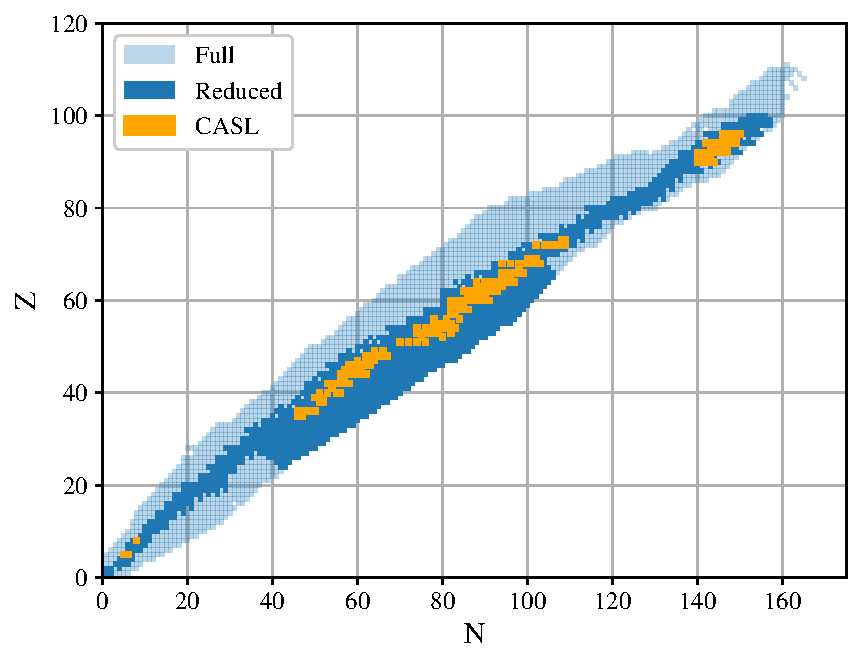
\includegraphics[width=4in]{figures/chains.pdf}
  \caption{Table of nuclides showing which nuclides are included in each of the
    depletion chains based on ENDF/B-VII.1.}
  \label{fig:chains}
\end{figure}

\subsubsection{Transmutation Reactions}

OpenMC will setup tallies in a problem based on what transmutation reactions are
available in a depletion chain file, so any arbitrary number of transmutation
reactions can be tracked. By default, the automatic depletion chain generation
described in \cref{sec:depletion-chain} will include the following transmutation
reactions: fission, (n,$\gamma$), (n,2n), (n,3n), (n,4n), (n,p), and
(n,$\alpha$). While this is suitable for fission applications, fusion
applications may require a wider set of transmutation reactions to be tracked.
Currently, reaction rates are determined by directly tallying the reaction rates
using a tracklength estimator.

\subsubsection{Capture Branching Ratios}

(n,$\gamma$) reactions may result in a product nucleus being in either the
ground state or an excited state. If the excited state is a metastable state
(having an unusually long half-life), it is important to account for this
difference during depletion. The most well-known example is capture in
$^{241}$Am, which can produce either $^{242}$Am or $^{242\text{m}}$Am. Because the
metastable state has a significantly longer half-life than the ground state, it
is important to account for the branching of the capture reaction in $^{241}$Am
to accurately predict the production of higher actinides~\citep{haeck2012nse}.
This is complicated by the fact that the branching ratio may depend on the
incident neutron energy causing capture.

OpenMC does not currently implement a method to handle energy-dependent capture
branching ratios directly. However, the depletion chain file does allow a
reaction to be listed multiple times with different branching ratios that result
in different products. Spectrum-averaged capture branching ratios have been
computed in LWR and SFR spectra and are available at
\url{https://openmc.org/depletion-chains}. Within the Python API, the class
representing a depletion chain allows branching ratios to be easily retrieved
and changed. We note that while this treatment doesn't accurately account for
the change in the capture branching ratio with increasing burnup (due to
spectral changes), these changes are generally much smaller than the differences
in capture branching ratios between nuclear data evaluations.

\subsubsection{Fission Product Yields}
\label{sec:fpy}

Like capture branching ratios, FPYs also depend on the incident neutron energy.
ENDF FPY sublibraries typically include yields tabulated at two or three
energies (thermal, fast, and fusion energies). Complicating matters is the fact
that while these data are specified for a single energy, they actually represent
the observed FPYs for a spectrum of energies (characterized by a single point).
For example, FPYs are often given at \SI{0.0253}{\electronvolt}, but this
actually represents the observed FPYs under a thermal neutron spectrum that
contains a continuum of energies. The ENDF-6 formats manual~\citep{trkov2018bnl}
recommends using linear-linear interpolation between energy points. However, at
the end of a transport solve, we typically have a one-group or multigroup
fission reaction rate---it's not clear how one should use this information to
calculate an effective FPY.

Different codes have adopted different approaches in how to handle the energy
dependence of FPYs. In ORIGEN, the average neutron energy causing fission is
calculated, and FPYs are interpolated using this average
energy~\citep{gauld2011nt}. In MCNP, the fission rate is tallied over a few
energy groups (thermal, fast, and high energy), and the energy group that
contains the majority of fissions is used to select appropriate
FPYs~\citep{fensin2008nt,fensin2011lanl}. In Serpent, a linear interpolation
factor is scored based on the neutron energy causing fission in relationship to
the energy points at which FPY are tabulated; the interpolation factor is then
used to calculate an effective FPY~\citep{kunchev2019mc}.

Rather than choose a single method, OpenMC includes three methods for treating
the energy dependence of FPYs. In the first method, FPY data corresponding to a
specific energy is manually selected. This approach may be appropriate if it is
known that neutrons in the system under consideration have a typical thermal,
fast, or fusion energy spectrum. In the second method, fission rates are tallied
above and below a specified cutoff energy. Then, thermal FPYs are used for all
fissions below the cutoff energy, and fast FPYs are used for all fissions above
the cutoff energy. In the third method, the average energy at which fission
events occur is tallied,
\begin{equation}
  \bar{E} = \frac{\int_0^\infty dE \; E \sigma_f(E)\phi(E)}{\int_0^\infty \sigma_f(E) \phi(E)},
\end{equation}
where $\sigma_f$ is the microscopic fission cross section and $\phi$ is the
neutron flux. An effective FPY is then calculated by linearly interpolating
between tabulated FPYs using the average energy. This approach is effectively
the same as that used by ORIGEN~\citep{gauld2011nt}.

\subsubsection{Power Normalization}

The reaction rates calculated by OpenMC are given in units of reactions per
source particle. For depletion, it is necessary to compute an absolute reaction
rate in reactions per second. To do so, the total observed heating in the system
is determined, and then the ratio of the system power to the observed heating is
used as a normalization factor on the reaction rates. OpenMC allows the total
heating to be determined by two different methods. In the first method, fission
reaction rates are multiplied by constant Q values in the depletion chain file
to estimate the total heating. This method is particularly useful for making
inter-code comparisons, where one must ensure that the same Q values for fission
are applied. In the second method, the actual heating rate is tallied over the
entire system (separate from the tally for transmutation reaction rates). This
method makes it possible to account for the energy dependence of the fission
energy release data as well as the fact that neutrons and photons may leak out
of the system, carrying away their energy with them. The latter effect may be
particularly important for small, leaky systems.

\subsection{Implementation}

OpenMC's core particle transport solver is written in C++ and is built as a
single executable. Most of the user-facing code, however, is written in Python.
Generally, to run OpenMC, a user writes a Python script that utilizes classes
and functions defined as part of an API to generate XML input files that are
then read by the executable. On top of this, OpenMC is also built as a shared
library with a C++ API that can be called by external programs. OpenMC's Python
API includes bindings to the C++ API; this enables a single run to be broken up
into individual components. For example, a function call from the Python
bindings to the C++ API can initialize the solver (reading inputs, loading cross
sections, etc.) without actually performing a simulation. A separate function
call can run the transport simulation. Further function calls allow a power user
to obtain information about tally results directly in memory from the C++ API.

OpenMC's depletion capability is implemented entirely in Python as the
\texttt{openmc.deplete} module. This module relies on the Python bindings to the
C++ API to initialize OpenMC, create tallies necessary for depletion, run
transport simulations, and obtain tally results. This approach has two primary
advantages. First, the time necessary to load cross sections is amortized
because it only has to be performed once, as opposed to once per transport
simulation. Second, using the Python bindings to the C++ API allows results to
be read directly in memory rather than using filesystem I/O, which helps to
minimizing overhead, particularly for large simulations.

The \texttt{openmc.deplete} module is designed with three key abstract classes
that represent the major components of the depletion solver. Each of the
abstract classes themselves defines an interface, that is, a set of methods that
a subclass must implement. First, the abstract \texttt{TransportOperator} class
represents a particle transport solver. Subclasses of \texttt{TransportOperator}
are required to implement a method that takes a list of nuclide densities to be
used in the problem and a system power and returns the $k$-eigenvalue and the
reaction rates resulting from the transport operator. Currently, there is a
single subclass of \texttt{TransportOperator} that interfaces with the Python
bindings to OpenMC's C++ API to call a transport solve and obtain reaction rates.
Once reaction rates are obtained, a separate depletion chain class (that is not
abstract) uses them to construct the burnup matrix, $\vect{A}$, based on the
data present in the depletion chain.

The abstract \texttt{DepSystemSolver} class represents a solver for
\cref{eq:depletion-matrix} when $\vect{A}$ is constant (a solver that can
evaluate \cref{eq:constant-A}). Subclasses of \texttt{DepSystemSolver} are
required to implement a method that takes the burnup matrix $\vect{A}$, an
initial density vector $\vect{n}_0$, and a timestep size, and returns the
resulting nuclide densities at the end of the step. The only subclass of
\texttt{DepSystemSolver} at present is \texttt{IPFCramSolver}, which implements
the IPF form of CRAM to evaluate \cref{eq:constant-A}. Because the CRAM method
requires solving multiple sparse linear systems, this class relies on the
third-party \texttt{scipy.sparse} package~\citep{virtanen2020nm} for performing
a sparse linear solve.

The abstract \texttt{Integrator} class represents a time integration method.
This class effectively orchestrates the coupled transport--depletion simulation.
Subclasses of \texttt{Integrator} are required to implement a method that takes
an initial vector of nuclide densities, reaction rates returned from an
operator, a time interval, and a power, and returns the resulting nuclide
densities at the end of the step. Thus, \texttt{Integrator} utilizes
\texttt{TransportOperator} in order to obtain reaction rates given $\vect{n}$,
and once the burnup matrix is constructed, it utilizes \texttt{DepSystemSolver}
to deplete with a constant $\vect{A}$ as many times as is necessary. One example
of a subclass of \texttt{Integrator} is \texttt{CECMIntegrator}, which
implements the CE/CM method.

The depletion system in OpenMC is designed to be modular. Although the only
transport operator that is implemented is the OpenMC transport solver itself,
the rest of the infrastructure (time integration methods, CRAM solver) does not
rely on anything specific to OpenMC's transport solver, so one could in
principle implement a class that utilizes a different transport solver (whether
that be another Monte Carlo code or a deterministic code). Similarly, although
\texttt{IPFCramSolver} is the only depletion system solver implemented, one
could replace it with a different solver, for example, a solver based on
backward differentiation formulas.

Lastly, we note that when multiple depletable materials are present in a problem
(thereby requiring multiple independent solutions of
\cref{eq:depletion-matrix}), the work is fully parallelized over the available
processes/threads. The third-party \texttt{mpi4py} Python package is used to
distribute the material compositions among the participating MPI processes.
Then, within each process, Python's \texttt{multiprocessing} standard-library
module is used to distribute materials among threads within a single MPI
process. This matches the distributed- and shared-memory parallelization scheme
used in OpenMC's transport solver, which relies on MPI and OpenMP.

%%%%%%%%%%%%%%%%%%%%%%%%%%%%%%%%%%%%%%%%%%%%%%%%%%%%%%%%%%%%%%%%%%%%%%%%%%%%%%%%
\section{Results}
\label{sec:results}

To validate the depletion solver in OpenMC, we have carried out simulations
using the \texttt{openmc.deplete} module as well as a developmental version of
Serpent 2.1.32 on two simple problems. The first problem is a pressurized water
reactor (PWR) pincell and the second problem is a single assembly of a
sodium-cooled fast reactor (SFR). These problems were selected to cover both
thermal and fast neutron spectra. While we had originally attempted to use
Serpent 2.1.31, preliminary comparisons between OpenMC and this version of
Serpent revealed significant differences in the predicted concentration of
$^{97}$Mo. This difference was found to be due to $^{97\text{m}}$Y having a
non-zero independent yield and a zero cumulative yield in the FPY sublibrary
file for $^{235}$U fission in ENDF/B-VII.1. The zero cumulative yield caused
Serpent 2.1.31 to ignore it altogether, which resulted in significantly less
production of $^{97}$Mo. The developmental version of Serpent 2.1.32 no longer
ignores this particular fission product despite the erroneous cumulative yield.

While comparison of simulation predictions to an experiment is a better means of
ensuring fitness for a particular application, it is not without downsides.
First, the presence of experimental uncertainties makes it hard to ascertain
whether small differences are attributable to the uncertainties or errors in the
code itself. In a cross-code comparison, if the same solution method and
fundamental nuclear data are being used in both codes, one expects to obtain the
same answer. Thus, even very minute differences may be indicative of a true
problem in the method implementation in one of the codes.

\subsection{Data Preparation}

Given the remarks above, it is of utmost importance to ensure that the same
nuclear data are being used in a cross-code comparison. For a depletion
simulation, we must ensure that the incident neutron cross sections and
secondary angle/energy distributions, radioactive decay data, and FPYs are the
same for both codes. In the simulations performed, all data was based on the
ENDF/B-VII.1 nuclear data library~\citep{chadwick2011nds}. Incident neutron
cross sections from the ENDF/B-VII.1 library processed by the LANL nuclear data
team~\citep{conlin2013lanl}, known as endf71x, were used for transport
simulations in both OpenMC and Serpent. Serpent is able to use the ACE files
from the endf71x library directly while OpenMC uses an HDF5 format that requires
conversion of the ACE files first. For the PWR pincell problem,
$S(\alpha,\beta)$ thermal scattering data is also needed for hydrogen in light
water; because Serpent does not yet handle the continuous representation used in
the ENDF71SaB library, the light water data from ENDF/B-VII.0 was used instead.
We note that the light water evaluation didn't actually change between
ENDF/B-VII.0 and ENDF/B-VII.1.

In Serpent, the depletion solver relies directly on ENDF decay and FPY
sublibrary files. Appropriate decay and FPY libraries for Serpent were thus
formed by concatenating the ENDF files directly from the ENDF/B-VII.1
distribution. For OpenMC, cases were run with the full, reduced, and CASL
depletion chains based on ENDF/B-VII.1 decay and FPY sublibrary files.

To ensure that OpenMC and Serpent perform power normalization in the same
manner, the default fission heating values from Serpent were used in OpenMC. By
default, the energy release per fission in $^{235}$U in Serpent is set to
\SI{202.27}{\mega\electronvolt}, and the values for other actinides are scaled
based on the Q value for fission listed in MF=3 in the ENDF evaluation. Without
the same heating values, the power normalization might result in OpenMC
depleting materials too quickly or too slowly relative to Serpent.

Serpent uses energy-independent capture branching ratios by default that are
based on the JEFF 3.1 activation file using a PWR flux spectrum. For the PWR
problem, these energy-independent branching ratios were used in OpenMC. For the
SFR problem, Serpent was used to first generate representative capture branching
ratios in the fast flux spectrum using Serpent's energy-dependent capture
branching ratio treatment. Then, the energy-independent branching ratios were
set in both Serpent and OpenMC.

\subsection{PWR Pincell}

The PWR pincell problem is a single 2.4\% enriched PWR pincell from the BEAVRS
benchmark~\citep{horelik2013mc,horelik2018mit}. Material compositions and
dimensions from the BEAVRS benchmark were used without modification. The pincell
extends to positive/negative infinity in the $z$ direction and has reflective
boundary conditions in the $x$ and $y$ directions. A linear heating rate of
\SI{174}{\watt\per\centi\meter} was used for power normalization. The pin was
depleted to 50 MWd/kg using the following burnup schedule:
\begin{itemize}
  \item A single 0.1 MWd/kg, 0.4 MWd/kg, and 0.5 MWd/kg timesteps;
  \item 1.0 MWd/kg timesteps out to a cumulative burnup of 10.0 MWd/kg;
  \item 2.5 MWd/kg timesteps out to a cumulative burnup of 50.0 MWd/kg.
\end{itemize}
The short timesteps at the beginning are used to accurately capture the buildup
of xenon isotopes. In both codes, the predictor method was used for time
integration. While the predictor method is the least accurate time integration
method, the purpose of the comparison is to confirm that OpenMC and Serpent
produce comparable results irrespective of the absolute values.

Five coupled transport--depletion simulations were carried out with OpenMC to test
a variety of combinations of depletion chains and methods for handling FPY
energy dependence:
\begin{enumerate}
  \item Full depletion chain, thermal FPYs
  \item Full depletion chain, interpolated FPYs
  \item Reduced depletion chain, interpolated FPYs
  \item CASL depletion chain, thermal FPYs
  %\item CASL depletion chain, FPYs based on cutoff method
  \item CASL depletion chain, interpolated FPYs
\end{enumerate}
Because Serpent doesn't have an option for changing the depletion chain or the
method for handling FPY energy dependence, a single coupled transport--depletion
simulation with Serpent was carried out. For all simulations, 20 inactive
batches, 200 active batches, and \num{4.0e6} particles per batch were used,
which resulted in an uncertainty on the effective multiplication factor of about
3--4 pcm.

\Cref{fig:pwr-keff} shows the difference between $k_\text{eff}$ calculated by
OpenMC and Serpent. The blue points correspond to results using the full
depletion chain, the red points correspond to points using the reduced chain,
and the green points correspond to results using the CASL chain. For each chain,
the use of interpolated FPYs is denoted by circles and thermal FPYs by x's. At
zero days, the difference in $k_\text{eff}$ between OpenMC and Serpent is not
statistically significant. As the burnup increases, the difference for the full
chain cases rises to about 20 pcm. The reduced chain case exhibits the exact
same behavior as the full chain as one would expect. Use of the CASL chain
results in a slightly larger difference between OpenMC and Serpent at 50 MWd/kg,
about 40 pcm. We also see that for both the full and CASL chains, changing the
method for handling FPY energy dependence doesn't appear to have much of an
effect on $k_\text{eff}$, which is primarily driven by the prediction of
actinide concentrations.
\begin{figure}[H]
  \centering
  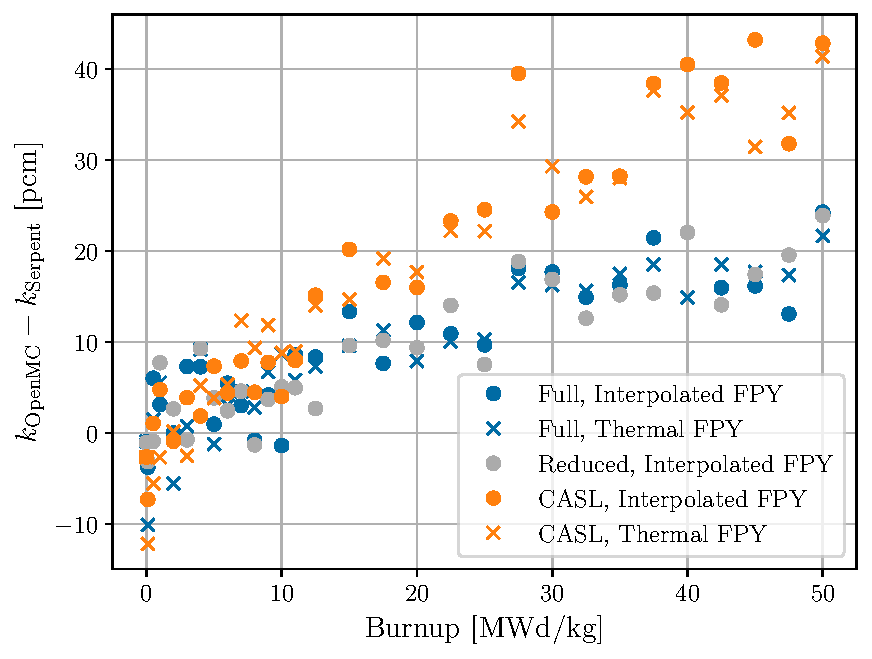
\includegraphics[width=4in]{figures/pwr_keff.pdf}
  \caption{Difference in the effective multiplication factor, $k_\text{eff}$,
  between OpenMC and Serpent for the PWR pincell model. While not shown, the one
  standard deviation uncertainty in the difference is about 3.5 pcm.}
  \label{fig:pwr-keff}
\end{figure}

\Cref{fig:pwr-actinides-full} shows the relative difference in predicted
actinide concentrations between OpenMC and Serpent at four different burnup
values. The fission products that are shown in \cref{fig:pwr-actinides-full}
have been chosen because they are either strong neutron absorbers or significant
contributors to decay heat and/or radiotoxicity. We see that most of the
differences are less than 0.1\%, and all are within 0.15\%. The differences in
$^{235}$U and $^{239}$Pu concentrations increase slightly with increasing
burnup, which most likely accounts for the 20 pcm difference observed for the
full chain in \cref{fig:pwr-keff}. While not shown, the predicted actinide
concentrations for the reduced chain are nearly identical to those observed for
the full chain in \cref{fig:pwr-actinides-full}. \Cref{fig:pwr-actinides-casl}
shows the differences in actinide concentrations using the CASL depletion chain.
Because the CASL depletion chain differs from the full depletion chain primarily
with respect to how fission products are treated, the differences reported in
\cref{fig:pwr-actinides-casl} closely mirror those in
\cref{fig:pwr-actinides-full}.
\begin{figure}[H]
  \centering
  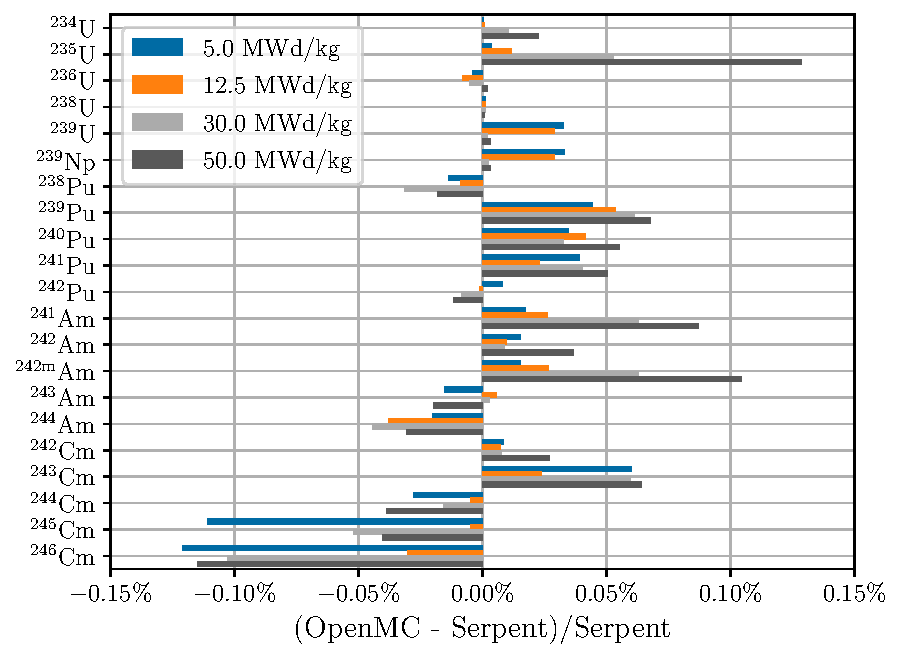
\includegraphics[width=4in]{figures/pwr_actinides_full.pdf}
  \caption{Relative difference in actinide concentrations between OpenMC and
  Serpent for the PWR pincell model at 5, 12.5, 30, and 50 MWd/kg using the full
  depletion chain.}
  \label{fig:pwr-actinides-full}
\end{figure}
\begin{figure}[H]
  \centering
  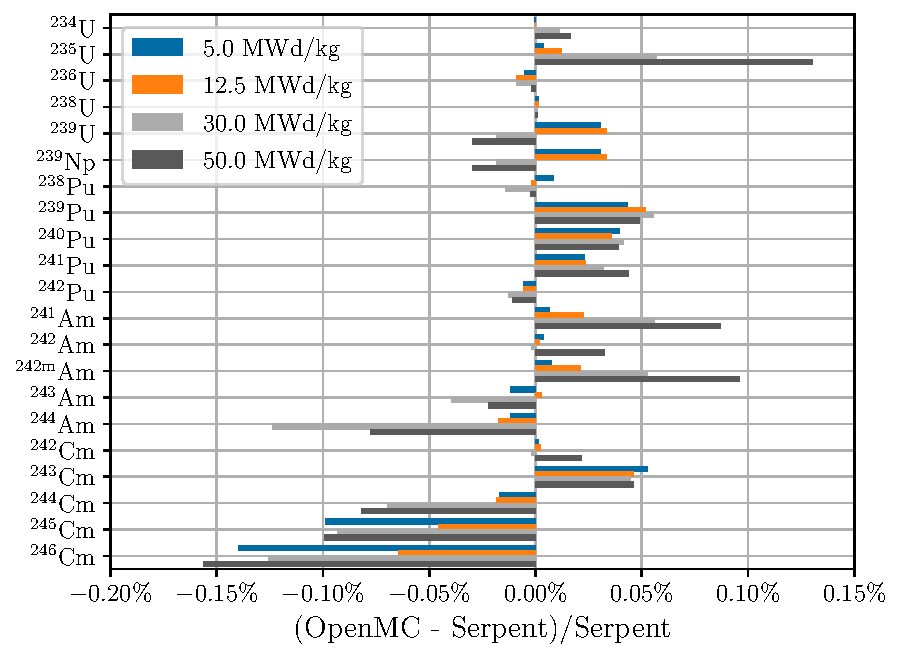
\includegraphics[width=4in]{figures/pwr_actinides_casl.pdf}
  \caption{Relative difference in actinide concentrations between OpenMC and
  Serpent for the PWR pincell model at 5, 12.5, 30, and 50 MWd/kg using the CASL
  depletion chain.}
  \label{fig:pwr-actinides-casl}
\end{figure}

The predicted concentration of fission products depends on both the depletion
chain that is used and the method for handling the energy dependence of the FPY.
We begin with results for the full depletion chain and interpolated FPYs, which
most closely matches the method used in Serpent; \cref{fig:pwr-fp-full-average}
shows the relative difference in fission product concentrations between OpenMC
and Serpent for this case. Most of the differences are less than 0.2\%, and only
a few fission products show differences up to 0.5\%.
\begin{figure}[H]
  \centering
  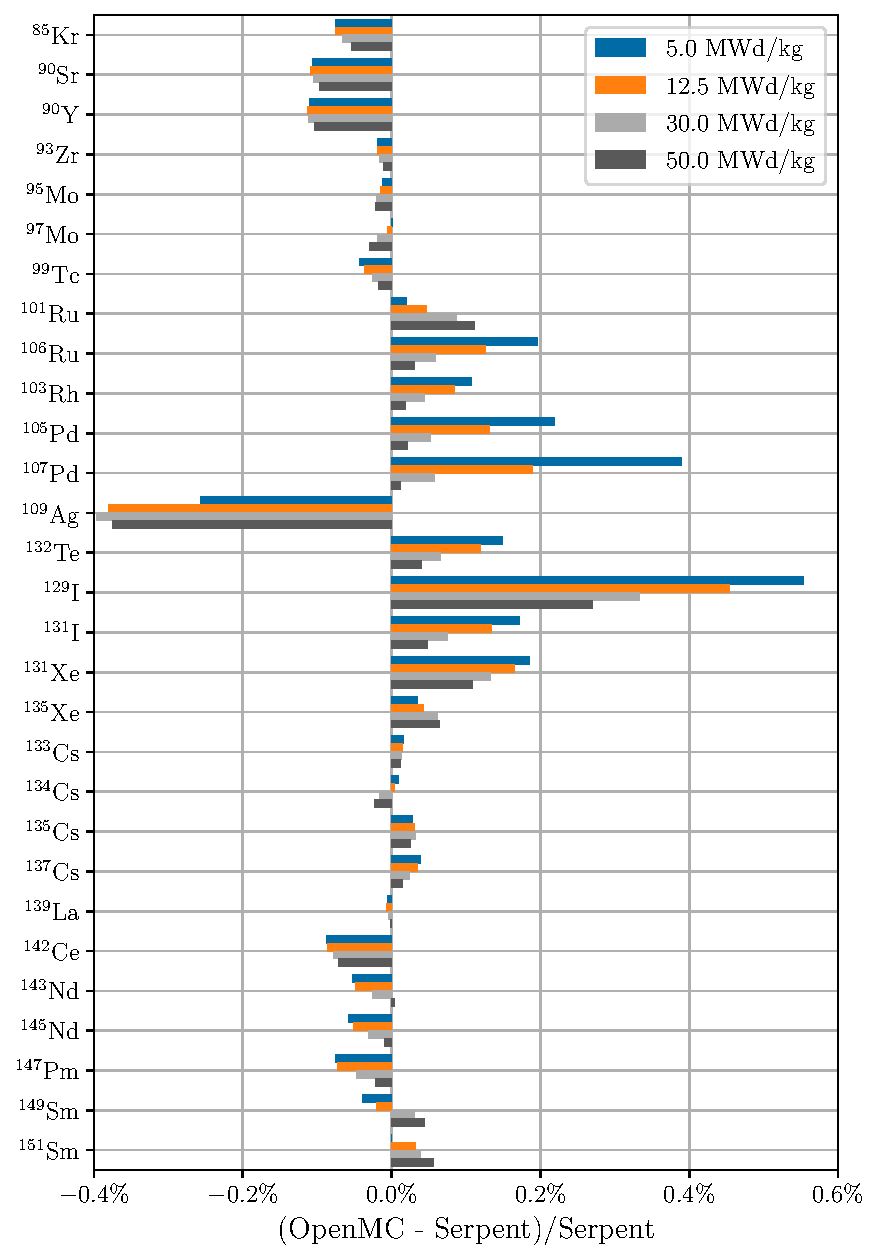
\includegraphics[width=4in]{figures/pwr_fp_full_average.pdf}
  \caption{Relative difference in fission product concentrations between OpenMC
  and Serpent for the PWR pincell model at 5, 12.5, 30, and 50 MWd/kg using the
  full depletion chain and interpolated FPYs.}
  \label{fig:pwr-fp-full-average}
\end{figure}

\Cref{fig:pwr-fp-full-thermal} shows the predicted fission product concentrations
when using the full depletion chain along with thermal FPYs. In this case,
although most fission products are within 1\% of Serpent, they are
systematically overpredicted other than a few nuclides. Because Serpent uses the
average fission energy to interpolate between two sets of FPYs, the systematic
difference is expected when using thermal FPYs in OpenMC. As the incident energy
of a neutron causing fission increases, the ``saddle'' and ``wings'' in the FPY
curve tend to increase significantly, and the peaks around $A=95$ and $A=135$
tend to slightly decrease. This corresponds to exactly what is observed in
\cref{fig:pwr-fp-full-thermal}. Because thermal FPYs were used in OpenMC for
this case, we expect that fission products near one of the two peaks of the FPY
curve will be slightly overpredicted relative to Serpent, and fission products
away from the peak will be underpredicted. This can be confirmed for particular
nuclides. Take, for example, $^{109}$Ag; in the $A=109$ mass chain, the nuclides
with the highest independent yields are $^{109}$Tc and $^{109}$Mo. Both these
nuclides have independent yields that increase significantly with increasing
neutron energy. The same situation occurs for $^{129}$I, whose predominant
precursor is $^{129}$Sn. The independent yields for these three precursor
nuclides are shown in \cref{tab:fp-yields}.
\begin{figure}[H]
  \centering
  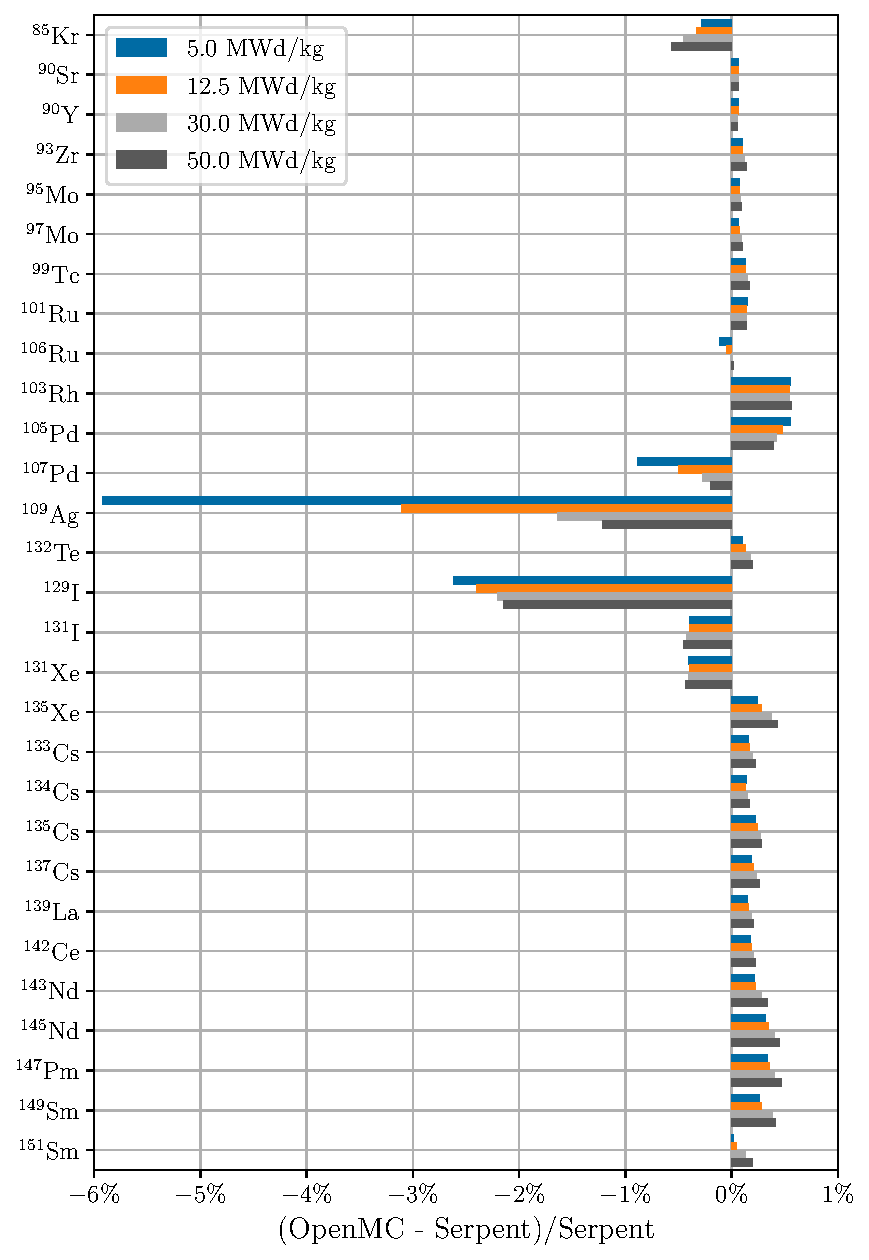
\includegraphics[width=4in]{figures/pwr_fp_full_thermal.pdf}
  \caption{Relative difference in fission product concentrations between OpenMC
  and Serpent for the PWR pincell model at 5, 12.5, 30, and 50 MWd/kg using the
  full depletion chain and thermal FPYs.}
  \label{fig:pwr-fp-full-thermal}
\end{figure}
\begin{table}[htbp]
  \centering
  \caption{Independent yields of select fission products due to fission in
  $^{235}$U (data from the ENDF/B-VII.1 FPY sublibrary).}
  \label{tab:fp-yields}
  \begin{tabular}{cccc}
    \toprule
    \textbf{Energy Spectrum} & \textbf{$^{109}$Tc} & \textbf{$^{109}$Mo} & \textbf{$^{129}$Sn} \\
    \midrule
    Thermal & 0.00013 & 0.00015 & 0.00230 \\
    Fast & 0.00034 & 0.00042 & 0.00550 \\
    Fusion & 0.00598 & 0.00109 & 0.01162 \\
    \bottomrule
  \end{tabular}
\end{table}

\Cref{fig:pwr-fp-casl-average} shows the relative difference in predicted
fission product concentrations between OpenMC and Serpent when using the CASL
depletion chain and interpolated FPYs. As in \cref{fig:pwr-fp-full-average},
almost all fission products are predicted to well within 1\% at 50 MWd/kg.
However, in this case there is one clear outlier: $^{85}$Kr. Upon further
investigation, it was determined that the root cause for this difference is the
fact that the CASL depletion chain uses a cumulative yield for $^{85}$Kr, and
the cumulative yield of $^{85}$Kr is known to be inconsistent with the
independent yields of the $A=85$ mass chain in
ENDF/B-VII.1~\citep{pigni2015nds}. Serpent relies solely on independent yields
in its depletion solver (as does the full depletion chain). We can conclude,
then, that there is nothing inherently wrong with the CASL depletion chain or
OpenMC; it is simply a matter of the underlying nuclear data being inconsistent.
The 5\% underprediction of $^{85}$Kr is also likely responsible for the slightly
higher difference in $k_\text{eff}$ for the CASL depletion chain shown in
\cref{fig:pwr-keff}.
\begin{figure}[H]
  \centering
  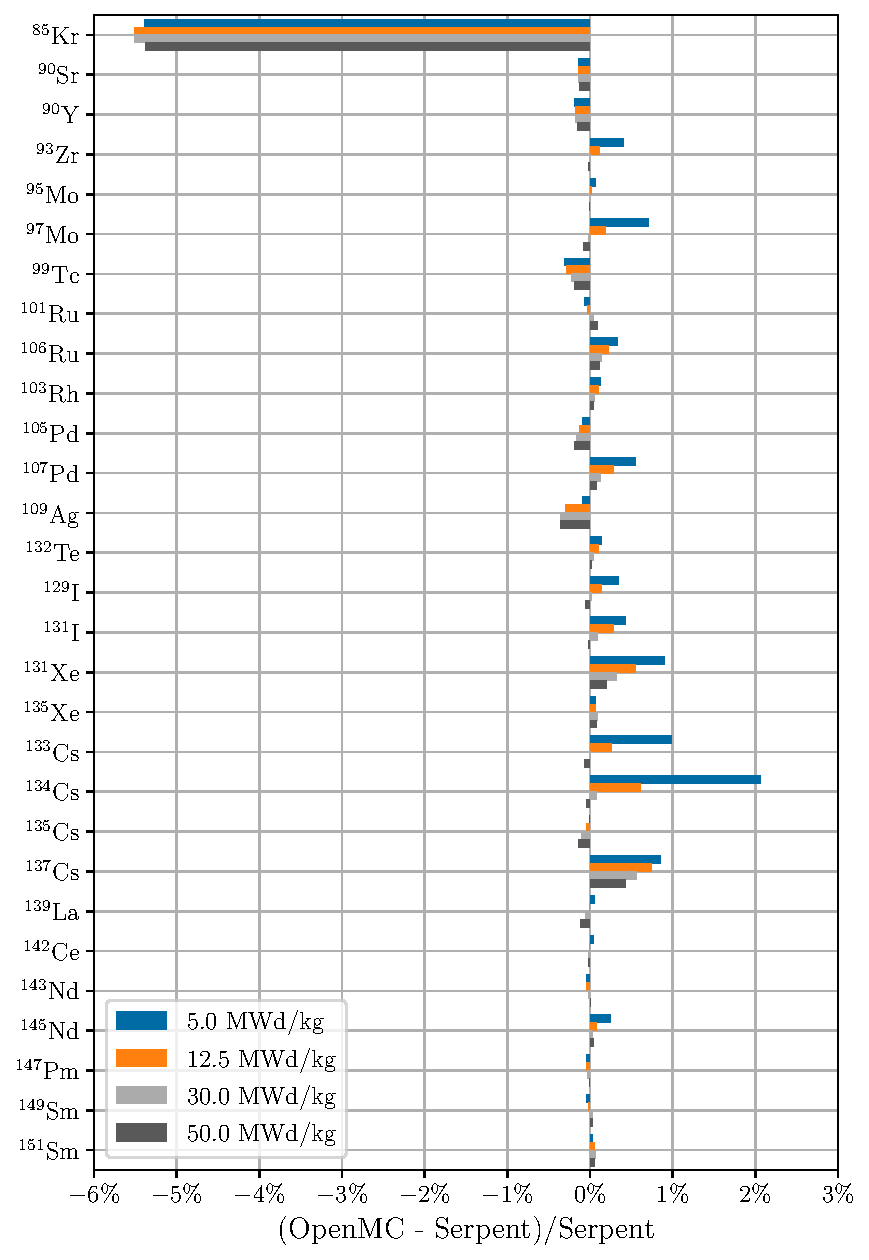
\includegraphics[width=4in]{figures/pwr_fp_casl_average.pdf}
  \caption{Relative difference in fission product concentrations between OpenMC
  and Serpent for the PWR pincell model at 5, 12.5, 30, and 50 MWd/kg using the
  CASL depletion chain and interpolated FPYs.}
  \label{fig:pwr-fp-casl-average}
\end{figure}

\Cref{fig:pwr-fp-casl-thermal} shows the relative difference in predicted in
fission product concentrations when using the CASL depletion chain along with
thermal FPYs. The results are quite close to those shown
\cref{fig:pwr-fp-full-thermal}, with the exception of $^{85}$Kr for the
aforementioned reasons.
\begin{figure}[H]
  \centering
  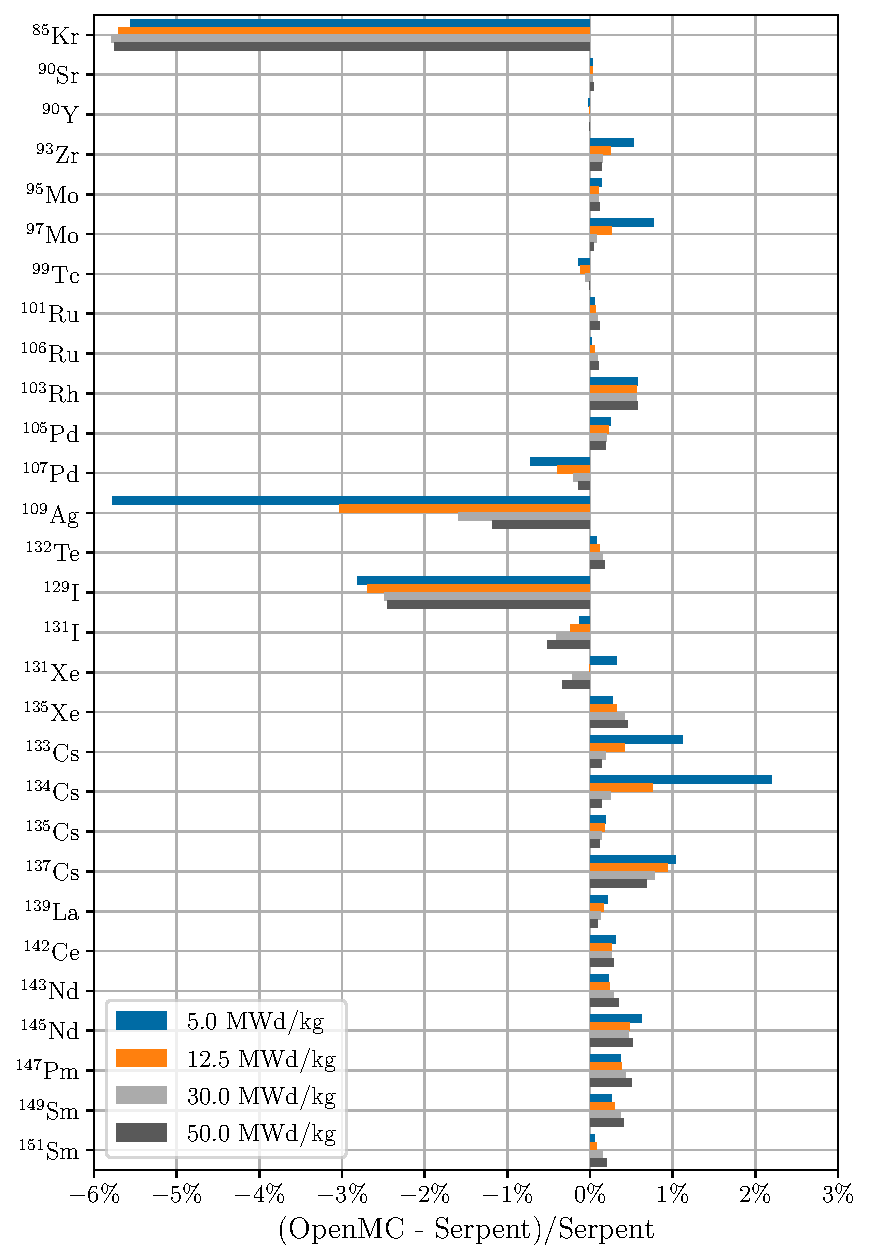
\includegraphics[width=4in]{figures/pwr_fp_casl_thermal.pdf}
  \caption{Relative difference in fission product concentrations between OpenMC
  and Serpent for the PWR pincell model at 5, 12.5, 30, and 50 MWd/kg using the
  CASL depletion chain and thermal FPYs.}
  \label{fig:pwr-fp-casl-thermal}
\end{figure}

\subsection{SFR Assembly}

The SFR assembly model is based on an OECD/NEA benchmark for SFR
analysis~\citep{nsc2015}. Namely, a 2D model of a driver assembly for the 1000
MWth metallic core (MET-1000) was used. The fuel composition corresponded to the
lowest axial region (the 17.16 cm column in Table 2.23 from ~\citep{nsc2015}).
All dimensions and material compositions can be found in the original OECD/NEA
report. The assembly model extends to positive/negative infinity in the $z$
direction and has periodic boundary conditions on the outer hexagonal surfaces.
A linear heating rate of \SI{23.3}{\kilo\watt\per\meter} per
pin~\citep{cahalan2007anl} was used for power normalization. The assembly was
depleted for 360 days in 20 day timesteps. As in the PWR pincell case, the
predictor method was used in both codes for time integration.

Unlike the PWR pincell model, which only contains materials at a single
temperature, the SFR assembly model uses a higher temperature in the fuel than
in other materials. In OpenMC, the temperature-dependence of neutron cross
sections was handled by interpolating data between neighboring temperatures.
Serpent uses an explicit temperature treatment known as target motion
sampling~\citep{viitanen2012nse}. However, we note that for this problem, the
temperature dependence of unresolved resonance probability tables becomes
important because of the fast flux spectrum, but the temperature treatment in
Serpent 2.1.31 does not handle probability tables.

Four coupled transport--depletion simulations were carried out with OpenMC for
the SFR assembly model:
\begin{enumerate}
  \item Full depletion chain, interpolated FPYs, probability tables on
  \item CASL depletion chain, interpolated FPYs, probability tables on
  \item Full depletion chain, interpolated FPYs, probability tables off
  \item CASL depletion chain, interpolated FPYs, probability tables off
\end{enumerate}
The results for the PWR pincell model indicated that the reduced depletion chain
results in identical behavior to the full depletion chain, so we have not
included a case for the SFR assembly using the reduced depletion chain. Two
coupled transport--depletion simulation with Serpent was carried out, one with
probability tables turned on and one with them turned off. For all simulations,
20 inactive batches, 200 active batches, and \num{4.0e6} particles per batch
were used, which resulted in an uncertainty on the effective multiplication
factor of 3--4 pcm.

% Also, we
% have only included a single case with thermal FPYs to compare with the use of
% interpolated FPYs using the same depletion chain.

\Cref{fig:sfr-keff} shows the difference between $k_\text{eff}$ calculated by
OpenMC and Serpent as the assembly is depleted. The blue points correspond to
results using the full depletion chain, and the green points correspond to
results using the CASL chain. For each chain, simulations with probability
tables on are denoted by circles and simulations without probability tables are
denoted by squares. Unlike in the PWR pincell case, there is a statistically
significant difference in $k_\text{eff}$ at zero days. Let us first consider the
case with probability tables turned off. In this case, $k_\text{eff}$ calculated
by OpenMC is about 20 pcm higher than that of Serpent. When using the full
depletion chain, there is no change in the difference between OpenMC and Serpent
with increasing burnup. When using the CASL depletion chain, the difference
increases by about 20--30 pcm, similar to the behavior shown in
\cref{fig:pwr-keff}. With probability tables turned on, however, the situation
is quite different. At zero days, $k_\text{eff}$ calculated by OpenMC is 20 pcm
lower than the value calculated by Serpent. As the burnup increases, there is an
increasing positive bias between OpenMC and Serpent. To understand the cause of
this difference, it is instructive to look at differences in isotopic
compositions.
\begin{figure}[H]
  \centering
  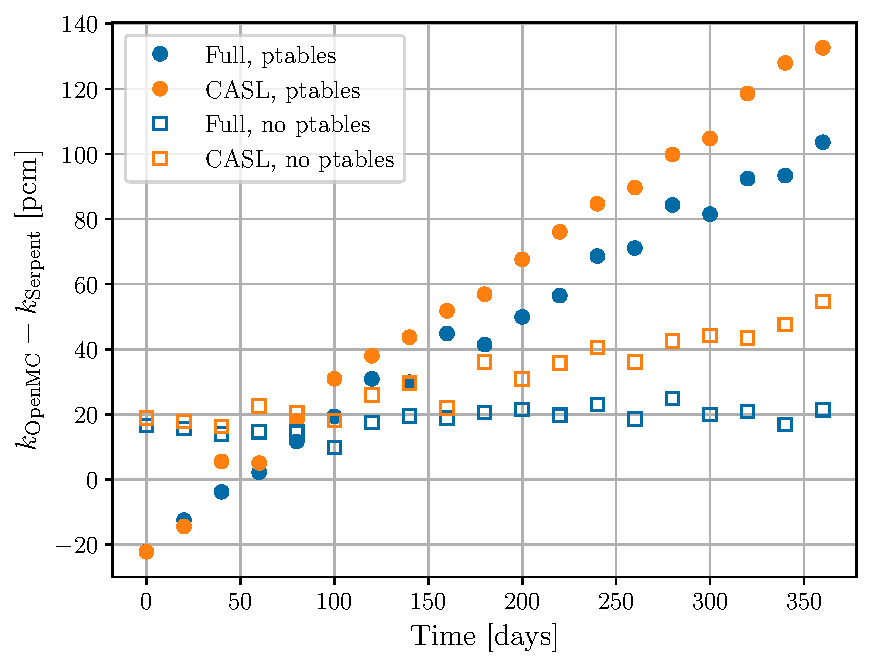
\includegraphics[width=4in]{figures/sfr_keff.pdf}
  \caption{Difference in the effective multiplication factor, $k_\text{eff}$,
  between OpenMC and Serpent for the SFR assembly model. While not shown, the one
  standard deviation uncertainty in the difference is about 3.5 pcm.}
  \label{fig:sfr-keff}
\end{figure}

\Cref{fig:sfr-actinides} shows the relative difference in predicted actinide
concentrations between OpenMC and Serpent with probability tables turned on. For
both the full and CASL depletion chains, the relative differences are all within
0.2\%. While this may seem close, the observed difference in $^{238}$U and
$^{239}$Pu concentrations merits special mention. In this model, the fuel
material is at \SI{807}{\kelvin}, but the endf71x library contains cross
sections processed at \SI{600}{\kelvin} and \SI{900}{\kelvin}. Thus, Serpent
ends up using probability tables at \SI{600}{\kelvin} rather than
\SI{807}{\kelvin}, which results in less parasitic absorption in $^{238}$U and
consequently less production of $^{239}$Pu (hence a lower $k_\text{eff}$ than
OpenMC with increasing burnup). Although OpenMC also does not have access to
probability tables at the exact fuel temperature, it statistically interpolates
between the probability tables at \SI{600}{\kelvin} and \SI{900}{\kelvin}.
\begin{figure}[H]
  \centering
  \begin{subfigure}[t]{0.45\textwidth}
    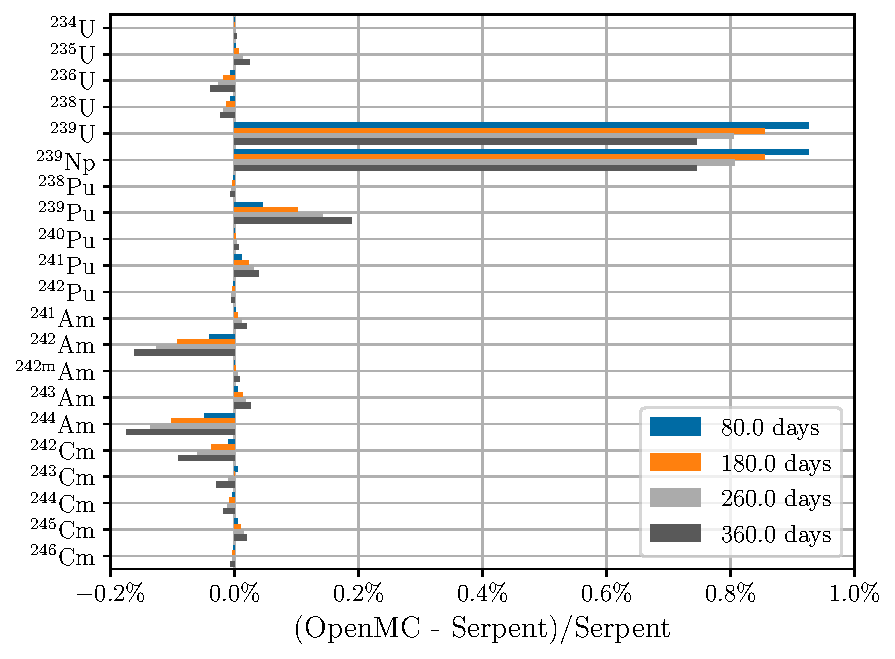
\includegraphics[width=\textwidth]{figures/sfr_actinides_full.pdf}
    \caption{Full depletion chain}
    \label{fig:sfr-actinides-full}
  \end{subfigure}
  \hspace{0.05\textwidth}
  \begin{subfigure}[t]{0.45\textwidth}
    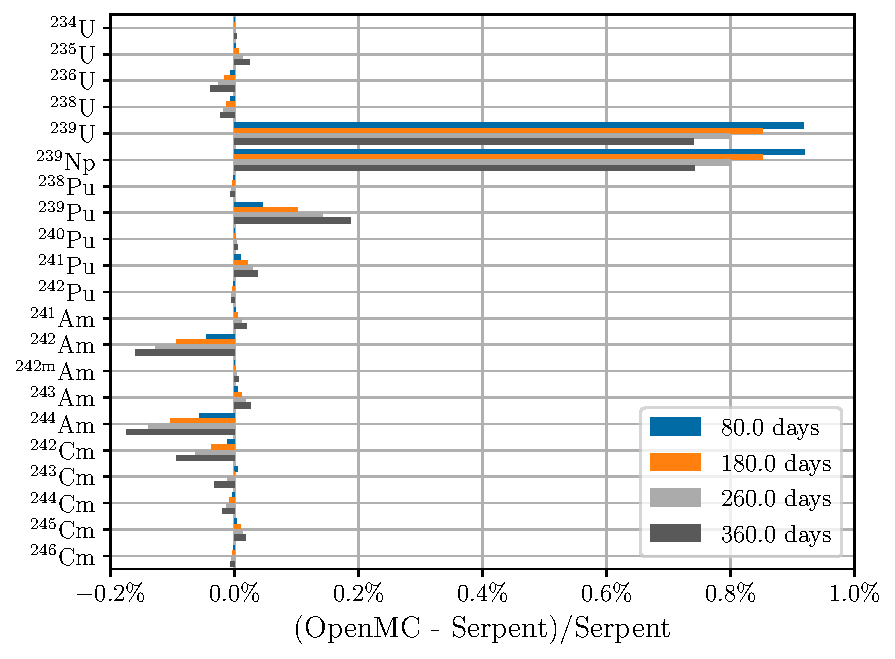
\includegraphics[width=\textwidth]{figures/sfr_actinides_casl.pdf}
    \caption{CASL depletion chain}
    \label{fig:sfr-actinides-casl}
  \end{subfigure}
  \caption{Relative difference in actinide concentrations between OpenMC and
  Serpent for the SFR assembly model at 80, 180, 260, and 360 days with
  probability tables on.}
  \label{fig:sfr-actinides}
\end{figure}

When probability tables are turned off, very close agreement is observed between
the predicted actinide concentrations in OpenMC and Serpent, as shown in
\cref{fig:sfr-actinides-nop}. In this case, the actinide concentrations agree to
within 0.01\% at all times during depletion for both the full and CASL depletion
chains.
\begin{figure}[H]
  \centering
  \begin{subfigure}[t]{0.45\textwidth}
    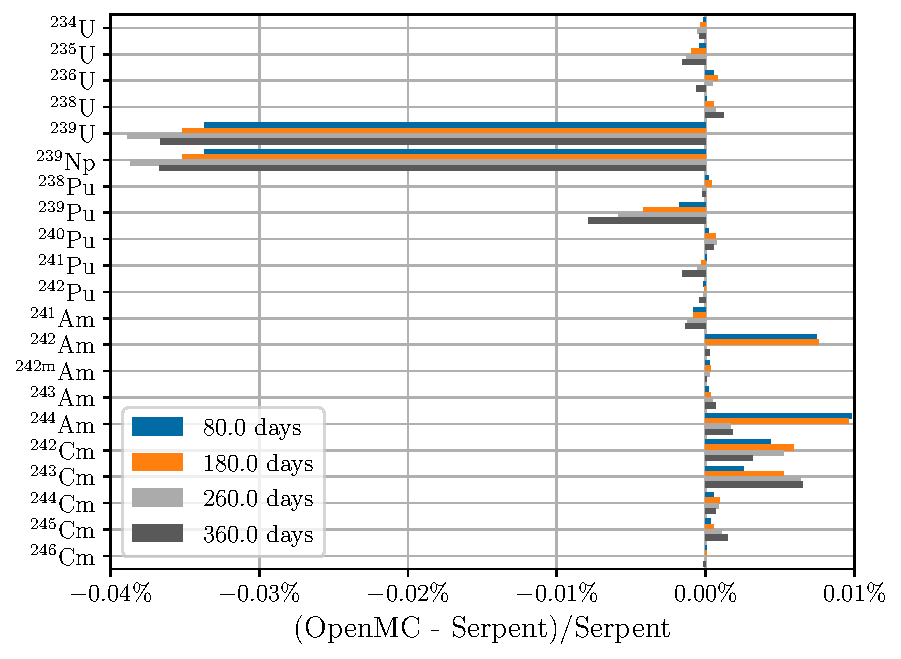
\includegraphics[width=\textwidth]{figures/sfr_actinides_full_nop.pdf}
    \caption{Full depletion chain}
    \label{fig:sfr-actinides-full-nop}
  \end{subfigure}
  \hspace{0.05\textwidth}
  \begin{subfigure}[t]{0.45\textwidth}
    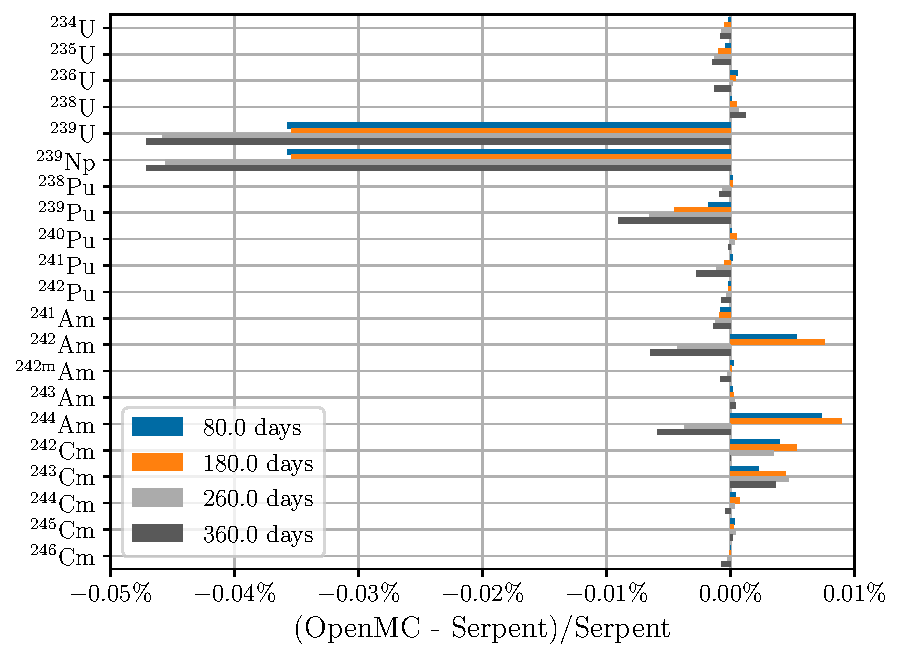
\includegraphics[width=\textwidth]{figures/sfr_actinides_casl_nop.pdf}
    \caption{CASL depletion chain}
    \label{fig:sfr-actinides-casl-nop}
  \end{subfigure}
  \caption{Relative difference in actinide concentrations between OpenMC and
  Serpent for the SFR assembly model at 80, 180, 260, and 360 days with
  probability tables off.}
  \label{fig:sfr-actinides-nop}
\end{figure}

\Cref{fig:sfr-fp} shows the relative difference in fission product
concentrations between OpenMC and Serpent with probability tables turned on.
Most differences between OpenMC and Serpent are below 1\%. As with the PWR
pincell model, OpenMC tends to produce a lower concentration of $^{109}$Ag most
likely because of differences in the treatment of FPY energy dependence. The
only noticeable difference between the full and CASL depletion chains is for
$^{85}$Kr, which is again explained by the use of an inconsistent cumulative
yield in the CASL depletion chain.
\begin{figure}[H]
  \centering
  \begin{subfigure}[t]{0.45\textwidth}
    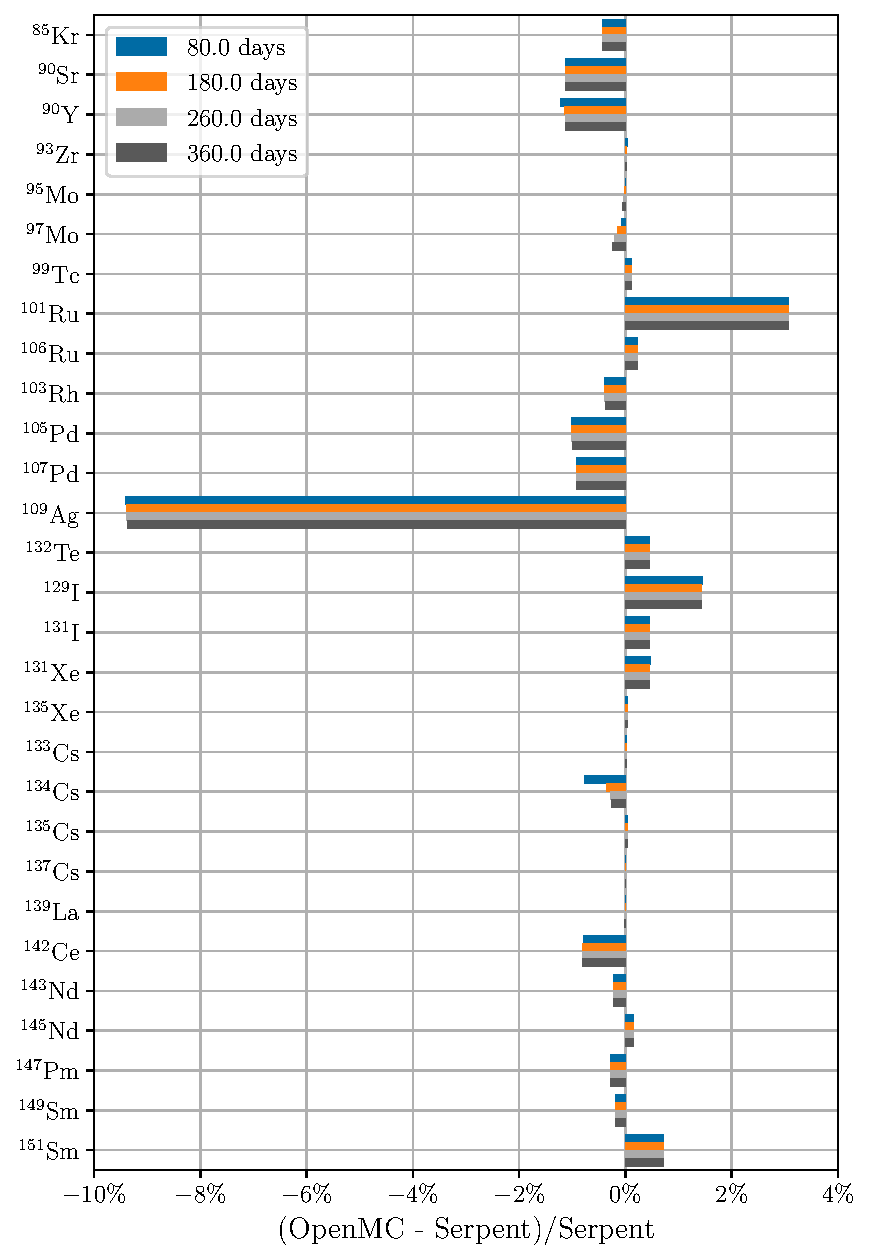
\includegraphics[width=\textwidth]{figures/sfr_fp_full_average.pdf}
    \caption{Full depletion chain}
  \end{subfigure}
  \hspace{0.05\textwidth}
  \begin{subfigure}[t]{0.45\textwidth}
    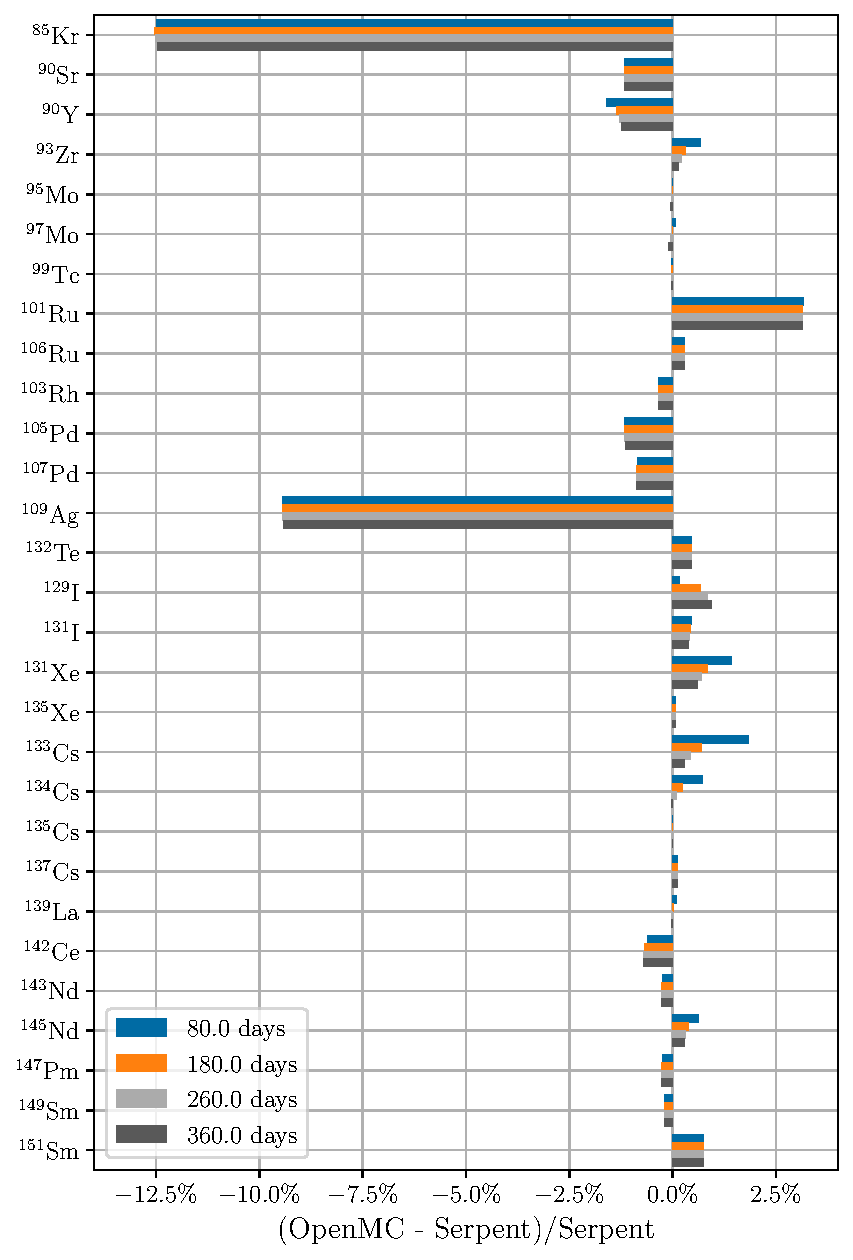
\includegraphics[width=\textwidth]{figures/sfr_fp_casl_average.pdf}
    \caption{CASL depletion chain}
  \end{subfigure}
  \caption{Relative difference in fission product concentrations between OpenMC
  and Serpent for the SFR assembly model at 80, 180, 260, and 360 days with
  probability tables on.}
  \label{fig:sfr-fp}
\end{figure}

With probability tables turned on, the differences between OpenMC and Serpent in
fission product concentrations are mostly the same as when probability tables
were turned off, as shown in \cref{fig:sfr-fp-nop}. Because the difference in
$^{238}$U and $^{239}$Pu concentrations was less than 0.2\% in
\cref{fig:sfr-actinides}, it makes sense that the use of probability tables
would not have a large effect on the fission product concentrations. Again, most
fission product concentrations agree to within 1\%, with $^{109}$Ag and
$^{85}$Kr being the notable outliers.
\begin{figure}[H]
  \centering
  \begin{subfigure}[t]{0.45\textwidth}
    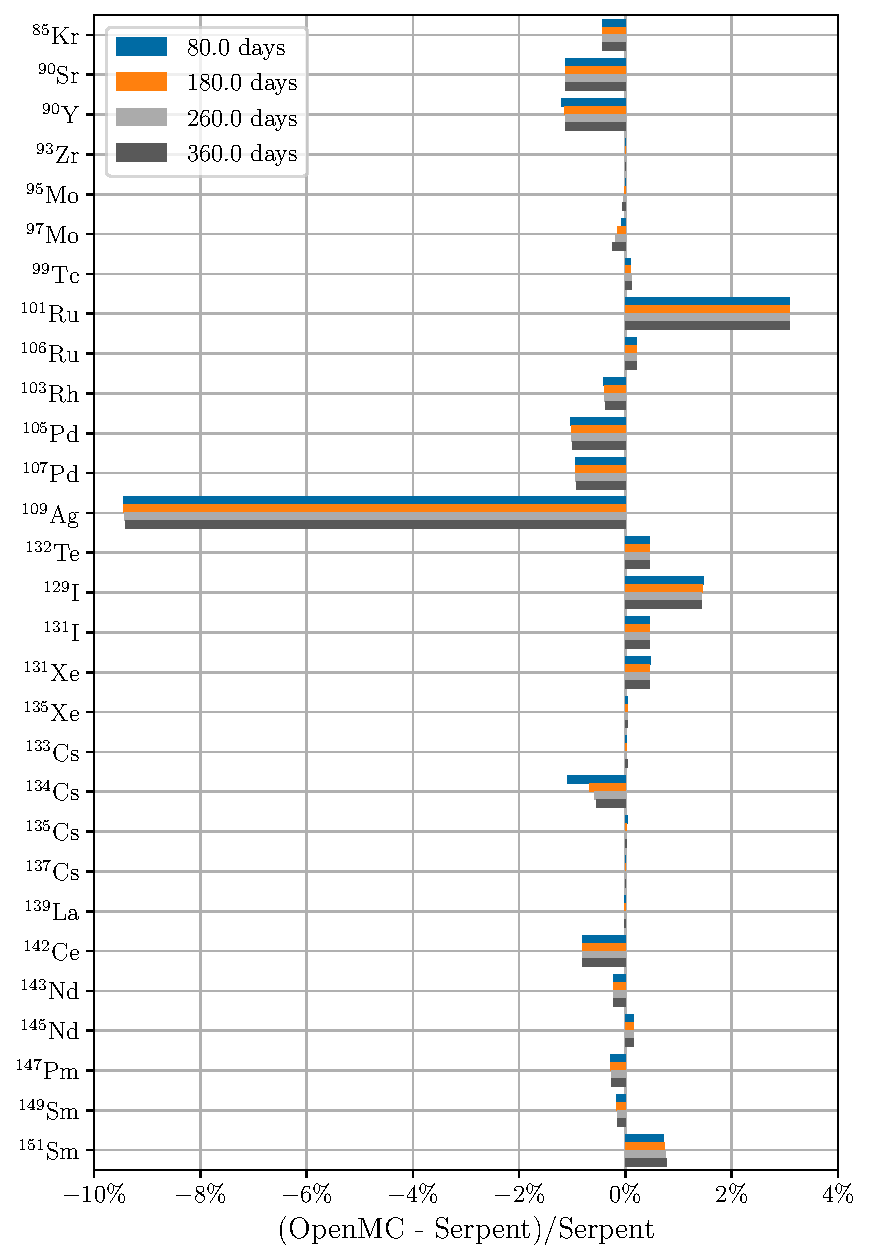
\includegraphics[width=\textwidth]{figures/sfr_fp_full_average_nop.pdf}
    \caption{Full depletion chain}
  \end{subfigure}
  \hspace{0.05\textwidth}
  \begin{subfigure}[t]{0.45\textwidth}
    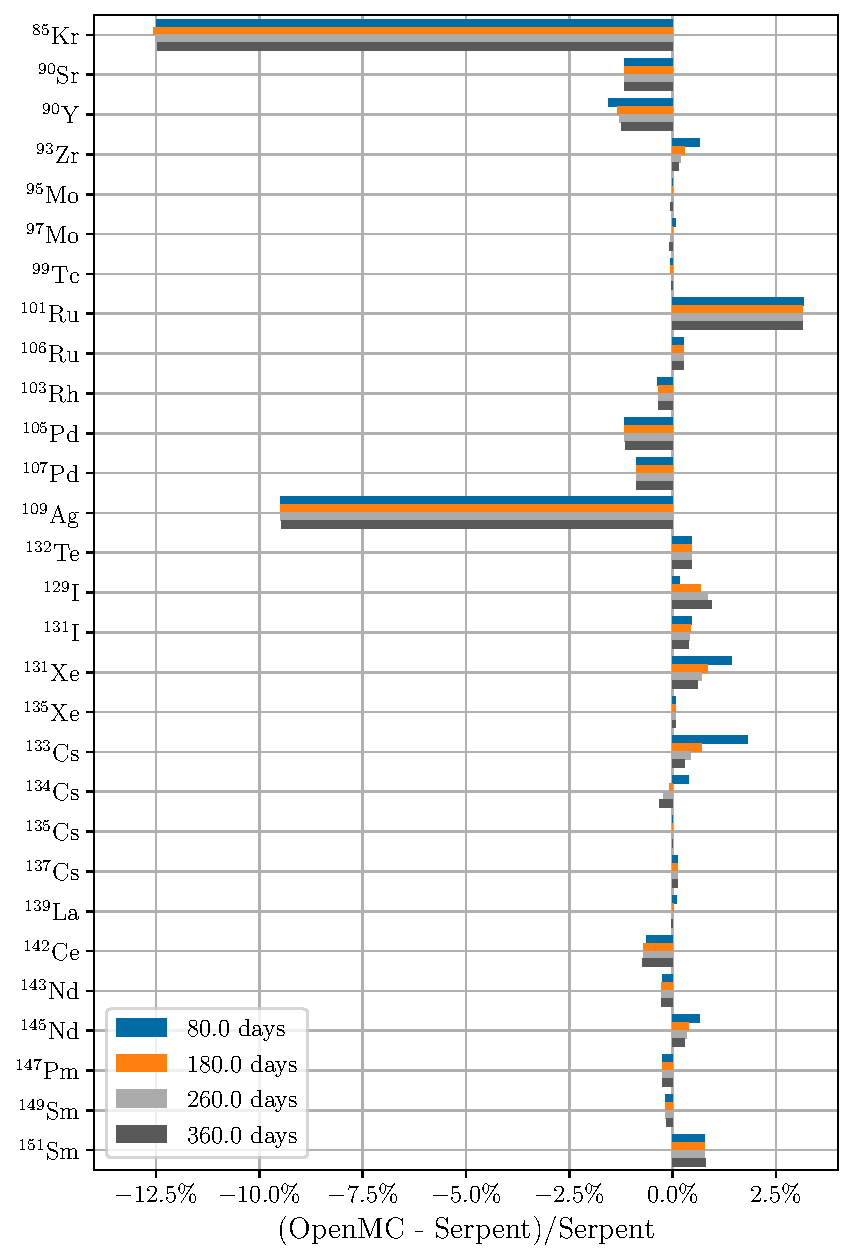
\includegraphics[width=\textwidth]{figures/sfr_fp_casl_average_nop.pdf}
    \caption{CASL depletion chain}
  \end{subfigure}
  \caption{Relative difference in fission product concentrations between OpenMC
  and Serpent for the SFR assembly model at 80, 180, 260, and 360 days with
  probability tables off.}
  \label{fig:sfr-fp-nop}
\end{figure}

%%%%%%%%%%%%%%%%%%%%%%%%%%%%%%%%%%%%%%%%%%%%%%%%%%%%%%%%%%%%%%%%%%%%%%%%%%%%%%%%
\section{Conclusions}
\label{sec:conclusions}

A new depletion solver has been implemented in the OpenMC Monte Carlo particle
transport code. The depletion solver is implemented primarily in Python 3 and
interfaces with OpenMC's transport solver through Python bindings to an
underlying C++ API, which enables data transfers to happen in memory rather than
through filesystem I/O. The design of the depletion solver relies on a set of
abstract classes that provide modularity and separation between different
components, including the time integration methods, the matrix exponential
solver, and the transport operator. In principle, this modularity would allow
the depletion system to be used with another transport code. Rather than relying
on a single time integration method, OpenMC implements several time integration
schemes including the predictor method, standard predictor--corrector methods,
stochastic implicit Euler integrators, and several novel
methods~\citep{josey2017phd, josey2017jcp}. To evaluate the matrix exponential,
OpenMC relies on the incomplete partial fraction form of CRAM by default.

To assess the accuracy of the new depletion solver, comparisons were made
between OpenMC and Serpent on a PWR pincell model and an SFR assembly model.
When the full depletion chain was used in OpenMC, the predictions of
$k_\text{eff}$ agreed to within 20--30 pcm of that calculated by Serpent at all
times in life for both the PWR and SFR model. Actinide concentrations were found
to agree to a fraction of a percent, and most fission product concentrations
were found to agree within 1\%. The few cases where fission product
concentrations differed by a larger amount were found to be related to
differences in the treatment of the energy dependence of FPYs. It is our sense
that there is no consensus in the community as to what is the ``correct'' way of
handling this energy dependence, so it is not possible to opine on whether one
set of results is right or wrong. When the simplified CASL depletion chain was
used in OpenMC, the accuracy of actinide and fission product concentrations did
not change appreciably. The only nuclide for which a significant difference was
observed was $^{85}$Kr; this difference can be explained by a cumulative yield
in the ENDF/B-VII.1 FPY sublibrary that is inconsistent with the independent
yields of precursors~\citep{pigni2015nds}. Because the CASL depletion chain
results in a significantly lower runtime compared to the full depletion chain
while still retaining accuracy, it is recommended for general use by OpenMC
users.

When comparing results on the SFR assembly model, larger differences in
$k_\text{eff}$ and isotopic concentrations were observed when unresolved
resonance region probability tables were turned on. These differences were found
to be related to how the temperature dependence of cross sections is treated in
the unresolved resonance region. In OpenMC, when the temperature of a material
is between two temperatures at which probability tables are tabulated,
statistical interpolation between the tables is performed. Serpent, on the other
hand, uses probability tables at the lower tabulated temperature. For the SFR
model, this results in lower parasitic neutron absorption in $^{238}$U, lower
production of $^{239}$Pu, and ultimately a lower $k_\text{eff}$. After depleting
for 360 days, there was a 100 pcm difference between OpenMC and Serpent due to
this effect. Although this is not a huge difference, users who are simulating
problems with a non-uniform temperature distribution should be aware of this
behavior.

Finally, we remark that although we did observe some differences between OpenMC
and Serpent, most of the differences were related to deficiencies in the nuclear
data itself. As a whole, the results demonstrate that when the same nuclear data
and same methods are used in two independently developed codes, it is possible
to obtain results in a depletion simulation that match within 10s of pcm on
$k_\text{eff}$ and less than 1\% on isotopic concentrations.

In the present work, we have only performed a cross-code comparison between
OpenMC and Serpent. While the results are certainly encouraging, we would
caution readers that no comparisons against experimental results have been
performed to date and would be needed to ensure the fitness for a particular
application. We also highlight the fact that the present comparisons are focused
solely on fission reactor applications. Although the \texttt{openmc.deplete}
module may eventually be of interest to other application areas, further changes
and enhancements would be needed. For example, for use in fusion applications, a
wider variety of transmutation reactions would need to be accounted for, and the
ability to handle transmutation from a fixed, pulsed neutron source would be
required.

%%%%%%%%%%%%%%%%%%%%%%%%%%%%%%%%%%%%%%%%%%%%%%%%%%%%%%%%%%%%%%%%%%%%%%%%%%%%%%%%
\section*{Acknowledgments}

We gratefully acknowledge the OpenMC user community for providing early feedback
and bug reports related to depletion that have helped improve the code. We wish
to acknowledge Jaakko Lepp{\"{a}}nen (VTT) for providing the developmental
version of Serpent 2.1.32 used in this work and for helping to shed light on the
methods used in Serpent. We acknowledge Nicolas Stauff (ANL) for providing
recommendations on a suitable SFR target problem.

This research was supported by the Exascale Computing Project (17-SC-20-SC), a
collaborative effort of the U.S. Department of Energy Office of Science and the
National Nuclear Security Administration. The submitted manuscript has been
created by UChicago Argonne, LLC, operator of Argonne National Laboratory under
contract DE-AC02-06CH11357.

We gratefully acknowledge the computing resources provided on Bebop, a
high-performance computing cluster operated by the Laboratory Computing Resource
Center at Argonne National Laboratory. This research made use of the resources
of the High Performance Computing Center at Idaho National Laboratory, which is
supported by the Office of Nuclear Energy of the U.S. Department of Energy and
the Nuclear Science User Facilities under Contract No. DE-AC07-05ID14517.

%%%%%%%%%%%%%%%%%%%%%%%%%%%%%%%%%%%%%%%%%%%%%%%%%%%%%%%%%%%%%%%%%%%%%%%%%%%%%%%%
%\section*{References}

\bibliographystyle{elsarticle-harv}
\bibliography{references}

\clearpage
\vspace*{\fill}
\noindent\fbox{%
  \parbox{\textwidth}{%
    The submitted manuscript has been created by UChicago Argonne, LLC, Operator
    of Argonne \mbox{National} Laboratory (``Argonne'').  Argonne, a
    U.S. Department of Energy Office of Science laboratory, is operated
    under Contract No. \mbox{DE-AC02-06CH11357}.  The U.S. Government retains for
    itself, and others acting on its behalf, a paid-up nonexclusive, irrevocable
    worldwide license in said article to reproduce, prepare derivative works,
    distribute copies to the public, and perform publicly and display publicly,
    by or on behalf of the Government. The Department of Energy will provide
    public access to these results of federally sponsored research in accordance
    with the DOE Public Access
    Plan. \url{http://energy.gov/downloads/doe-public-access-plan.}
  }%
}
\vspace*{\fill}

\end{document}
